\documentclass[aspectratio=169]{beamer}\usepackage[]{graphicx}\usepackage[]{xcolor}
% maxwidth is the original width if it is less than linewidth
% otherwise use linewidth (to make sure the graphics do not exceed the margin)
\makeatletter
\def\maxwidth{ %
  \ifdim\Gin@nat@width>\linewidth
    \linewidth
  \else
    \Gin@nat@width
  \fi
}
\makeatother

\definecolor{fgcolor}{rgb}{0.345, 0.345, 0.345}
\newcommand{\hlnum}[1]{\textcolor[rgb]{0.686,0.059,0.569}{#1}}%
\newcommand{\hlsng}[1]{\textcolor[rgb]{0.192,0.494,0.8}{#1}}%
\newcommand{\hlcom}[1]{\textcolor[rgb]{0.678,0.584,0.686}{\textit{#1}}}%
\newcommand{\hlopt}[1]{\textcolor[rgb]{0,0,0}{#1}}%
\newcommand{\hldef}[1]{\textcolor[rgb]{0.345,0.345,0.345}{#1}}%
\newcommand{\hlkwa}[1]{\textcolor[rgb]{0.161,0.373,0.58}{\textbf{#1}}}%
\newcommand{\hlkwb}[1]{\textcolor[rgb]{0.69,0.353,0.396}{#1}}%
\newcommand{\hlkwc}[1]{\textcolor[rgb]{0.333,0.667,0.333}{#1}}%
\newcommand{\hlkwd}[1]{\textcolor[rgb]{0.737,0.353,0.396}{\textbf{#1}}}%
\let\hlipl\hlkwb

\usepackage{framed}
\makeatletter
\newenvironment{kframe}{%
 \def\at@end@of@kframe{}%
 \ifinner\ifhmode%
  \def\at@end@of@kframe{\end{minipage}}%
  \begin{minipage}{\columnwidth}%
 \fi\fi%
 \def\FrameCommand##1{\hskip\@totalleftmargin \hskip-\fboxsep
 \colorbox{shadecolor}{##1}\hskip-\fboxsep
     % There is no \\@totalrightmargin, so:
     \hskip-\linewidth \hskip-\@totalleftmargin \hskip\columnwidth}%
 \MakeFramed {\advance\hsize-\width
   \@totalleftmargin\z@ \linewidth\hsize
   \@setminipage}}%
 {\par\unskip\endMakeFramed%
 \at@end@of@kframe}
\makeatother

\definecolor{shadecolor}{rgb}{.97, .97, .97}
\definecolor{messagecolor}{rgb}{0, 0, 0}
\definecolor{warningcolor}{rgb}{1, 0, 1}
\definecolor{errorcolor}{rgb}{1, 0, 0}
\newenvironment{knitrout}{}{} % an empty environment to be redefined in TeX

\usepackage{alltt}




\usetheme{default}
% Slide setup, colour independent

\usepackage{amsmath,amssymb,amsthm}
\usepackage[utf8]{inputenc}
\usepackage{colortbl}
\usepackage{bm}
\usepackage{xcolor}
\usepackage{dsfont}
\usepackage{setspace}
%\usepackage{subfigure}
% To use \ding{234} and the like
\usepackage{pifont}
% To cross reference between slide files
\usepackage{zref-xr,zref-user}
% Use something like
% \zexternaldocument{fileI}
% in the tex files. And cite using \zref instead of \ref
\usepackage{booktabs}

%\usepackage{transparent}

% Fields and the like
\def\IC{\mathbb{C}}
\def\IF{\mathbb{F}}
\def\II{\mathbb{I}}
\def\IJ{\mathbb{J}}
\def\IM{\mathbb{M}}
\def\IN{\mathbb{N}}
\def\IP{\mathbb{P}}
\def\IR{\mathbb{R}}
\def\IZ{\mathbb{Z}}
\def\11{\mathds{1}}


% Bold lowercase
\def\ba{\bm{a}}
\def\bb{\bm{b}}
\def\bc{\bm{c}}
\def\bd{\bm{d}}
\def\be{\bm{e}}
\def\bf{\bm{f}}
\def\bh{\bm{h}}
\def\bi{\bm{i}}
\def\bj{\bm{j}}
\def\bk{\bm{k}}
\def\bn{\bm{n}}
\def\bp{\bm{p}}
\def\br{\bm{r}}
\def\bs{\bm{s}}
\def\bu{\bm{u}}
\def\bv{\bm{v}}
\def\bw{\bm{w}}
\def\bx{\bm{x}}
\def\by{\bm{y}}
\def\bz{\bm{z}}

% Bold capitals
\def\bB{\bm{B}}
\def\bD{\bm{D}}
\def\bE{\bm{E}}
\def\bF{\bm{F}}
\def\bG{\bm{G}}
\def\bI{\bm{I}}
\def\bL{\bm{L}}
\def\bN{\bm{N}}
\def\bP{\bm{P}}
\def\bR{\bm{R}}
\def\bS{\bm{S}}
\def\bT{\bm{T}}
\def\bX{\bm{X}}

% Bold numbers
\def\b0{\bm{0}}

% Bold greek
\bmdefine{\bmu}{\bm{\mu}}
\def\bphi{\bm{\phi}}
\def\bvarphi{\bm{\varphi}}
\def\bPi{\bm{\Pi}}
\def\bGamma{\bm{\Gamma}}

% Bold red sentence
\def\boldred#1{{\color{red}\textbf{#1}}}
\def\defword#1{{\color{orange}\textbf{#1}}}

% Caligraphic letters
\def\A{\mathcal{A}}
\def\B{\mathcal{B}}
\def\C{\mathcal{C}}
\def\D{\mathcal{D}}
\def\E{\mathcal{E}}
\def\F{\mathcal{F}}
\def\G{\mathcal{G}}
\def\H{\mathcal{H}}
\def\I{\mathcal{I}}
\def\L{\mathcal{L}}
\def\M{\mathcal{M}}
\def\N{\mathcal{N}}
\def\P{\mathcal{P}}
\def\R{\mathcal{R}}
\def\S{\mathcal{S}}
\def\T{\mathcal{T}}
\def\U{\mathcal{U}}
\def\V{\mathcal{V}}

% Adding space for prime (') where needed
\def\pprime{\,'}
% Adding space for star (\star) where needed
\def\pstar{{\,\star}}

% tt font for code
\def\code#1{{\tt #1}}

% i.e., e.g.
\def\eg{\emph{e.g.}}
\def\ie{\emph{i.e.}}


% Operators and special symbols
\def\nbOne{{\mathchoice {\rm 1\mskip-4mu l} {\rm 1\mskip-4mu l}
{\rm 1\mskip-4.5mu l} {\rm 1\mskip-5mu l}}}
\def\cov{\ensuremath{\mathsf{cov}}}
\def\Var{\ensuremath{\mathsf{Var}\ }}
\def\Im{\textrm{Im}\;}
\def\Re{\textrm{Re}\;}
\def\det{\ensuremath{\mathsf{det}}}
\def\diag{\ensuremath{\mathsf{diag}}}
\def\nullspace{\ensuremath{\mathsf{null}}}
\def\nullity{\ensuremath{\mathsf{nullity}}}
\def\rank{\ensuremath{\mathsf{rank}}}
\def\range{\ensuremath{\mathsf{range}}}
\def\sgn{\ensuremath{\mathsf{sgn}}}
\def\Span{\ensuremath{\mathsf{span}}}
\def\tr{\ensuremath{\mathsf{tr}}}
\def\imply{$\Rightarrow$}
\def\restrictTo#1#2{\left.#1\right|_{#2}}
\newcommand{\parallelsum}{\mathbin{\!/\mkern-5mu/\!}}
\def\dsum{\mathop{\displaystyle \sum }}%
\def\dind#1#2{_{\substack{#1\\ #2}}}

\DeclareMathOperator{\GL}{GL}
\DeclareMathOperator{\Rel}{Re}
\def\Nt#1{\left|\!\left|\!\left|#1\right|\!\right|\!\right|}
\newcommand{\tripbar}{|\! |\! |}



% The beamer bullet (in base colour)
\def\bbullet{\leavevmode\usebeamertemplate{itemize item}\ }

% Theorems and the like
\newtheorem{proposition}[theorem]{Proposition}
\newtheorem{property}[theorem]{Property}
\newtheorem{importantproperty}[theorem]{Property}
\newtheorem{importanttheorem}[theorem]{Theorem}
%\newtheorem{lemma}[theorem]{Lemma}
%\newtheorem{corollary}[theorem]{Corollary}
\newtheorem{remark}[theorem]{Remark}
\setbeamertemplate{theorems}[numbered]
%\setbeamertemplate{theorems}[ams style]

%
%\usecolortheme{orchid}
%\usecolortheme{orchid}

\def\red{\color[rgb]{1,0,0}}
\def\blue{\color[rgb]{0,0,1}}
\def\green{\color[rgb]{0,1,0}}


% Get rid of navigation stuff
\setbeamertemplate{navigation symbols}{}

% Set footline/header line
\setbeamertemplate{footline}
{%
\quad p. \insertpagenumber \quad--\quad \insertsection\vskip2pt
}
% \setbeamertemplate{headline}
% {%
% \quad\insertsection\hfill p. \insertpagenumber\quad\mbox{}\vskip2pt
% }


\makeatletter
\newlength\beamerleftmargin
\setlength\beamerleftmargin{\Gm@lmargin}
\makeatother

% Colours for special pages
\def\extraContent{yellow!20}


%%%%%%%%%%%%%%%%%
\usepackage{tikz}
\usetikzlibrary{shapes,arrows}
\usetikzlibrary{positioning}
\usetikzlibrary{shapes.symbols,shapes.callouts,patterns}
\usetikzlibrary{calc,fit}
\usetikzlibrary{backgrounds}
\usetikzlibrary{decorations.pathmorphing,fit,petri}
\usetikzlibrary{automata}
\usetikzlibrary{fadings}
\usetikzlibrary{patterns,hobby}
\usetikzlibrary{backgrounds,fit,petri}


\usepackage{pgfplots}
\pgfplotsset{compat=1.6}
\pgfplotsset{ticks=none}

\usetikzlibrary{decorations.markings}
\usetikzlibrary{arrows.meta}
\tikzset{>=stealth}

% For tikz
\tikzstyle{cloud} = [draw, ellipse,fill=red!20, node distance=0.87cm,
minimum height=2em]
\tikzstyle{line} = [draw, -latex']


%%% For max frame images
\newenvironment{changemargin}[2]{%
\begin{list}{}{%
\setlength{\topsep}{0pt}%
\setlength{\leftmargin}{#1}%
\setlength{\rightmargin}{#2}%
\setlength{\listparindent}{\parindent}%
\setlength{\itemindent}{\parindent}%
\setlength{\parsep}{\parskip}%
}%
\item[]}{\end{list}}


% Make one image take up the entire slide content area in beamer,.:
% centered/centred full-screen image, with title:
% This uses the whole screen except for the 1cm border around it
% all. 128x96mm
\newcommand{\titledFrameImage}[2]{
\begin{frame}{#1}
%\begin{changemargin}{-1cm}{-1cm}
\begin{center}
\includegraphics[width=108mm,height=\textheight,keepaspectratio]{#2}
\end{center}
%\end{changemargin}
\end{frame}
}

% Make one image take up the entire slide content area in beamer.:
% centered/centred full-screen image, no title:
% This uses the whole screen except for the 1cm border around it
% all. 128x96mm
\newcommand{\plainFrameImage}[1]{
\begin{frame}[plain]
%\begin{changemargin}{-1cm}{-1cm}
\begin{center}
\includegraphics[width=108mm,height=76mm,keepaspectratio]{#1}
\end{center}
%\end{changemargin}
\end{frame}
}

% Make one image take up the entire slide area, including borders, in beamer.:
% centered/centred full-screen image, no title:
% This uses the entire whole screen
\newcommand{\maxFrameImage}[1]{
\begin{frame}[plain]
\begin{changemargin}{-1cm}{-1cm}
\begin{center}
\includegraphics[width=\paperwidth,height=\paperheight,keepaspectratio]
{#1}
\end{center}
\end{changemargin}
\end{frame}
}

% This uses the entire whole screen (to include in frame)
\newcommand{\maxFrameImageNoFrame}[1]{
\begin{changemargin}{-1cm}{-1cm}
\begin{center}
\includegraphics[width=\paperwidth,height=0.99\paperheight,keepaspectratio]
{#1}
\end{center}
\end{changemargin}
}

% Make one image take up the entire slide area, including borders, in beamer.:
% centered/centred full-screen image, no title:
% This uses the entire whole screen
\newcommand{\maxFrameImageColor}[2]{
\begin{frame}[plain]
\setbeamercolor{normal text}{bg=#2!20}
\begin{changemargin}{-1cm}{-1cm}
\begin{center}
\includegraphics[width=\paperwidth,height=\paperheight,keepaspectratio]
{#1}
\end{center}
\end{changemargin}
\end{frame}
}


\usepackage{tikz}
\usetikzlibrary{patterns,hobby}
\usepackage{pgfplots}
\pgfplotsset{compat=1.6}
\pgfplotsset{ticks=none}

\usetikzlibrary{backgrounds}
\usetikzlibrary{decorations.markings}
\usetikzlibrary{arrows.meta}
\tikzset{>=stealth}

\tikzset{
  clockwise arrows/.style={
    postaction={
      decorate,
      decoration={
        markings,
        mark=between positions 0.1 and 0.9 step 40pt with {\arrow{>}},
   }}}}


   %%%%%%%%%%%
% To have links to parts in the outline
\makeatletter
\AtBeginPart{%
  \addtocontents{toc}{\protect\beamer@partintoc{\the\c@part}{\beamer@partnameshort}{\the\c@page}}%
}
%% number, shortname, page.
\providecommand\beamer@partintoc[3]{%
  \ifnum\c@tocdepth=-1\relax
    % requesting onlyparts.
    \makebox[6em]{Part #1:} \textcolor{green!30!blue}{\hyperlink{#2}{#2}}
    \par
  \fi
}
\define@key{beamertoc}{onlyparts}[]{%
  \c@tocdepth=-1\relax
}
\makeatother%

\newcommand{\nameofthepart}{}
\newcommand{\nupart}[1]%
    {   \part{#1}%
        \renewcommand{\nameofthepart}{#1}%
        {
          \setbeamercolor{background canvas}{bg=orange!50}
          \begin{frame}{#1}%\partpage 
          \hypertarget{\nameofthepart}{}\tableofcontents%
          \end{frame}
        }
    }



\usecolortheme{orchid}
%% Listings
\usepackage{listings}
\definecolor{mygreen}{rgb}{0,0.6,0}
\definecolor{mygray}{rgb}{0.5,0.5,0.5}
\definecolor{mymauve}{rgb}{0.58,0,0.82}
\definecolor{mygold}{rgb}{1,0.843,0}
\definecolor{myblue}{rgb}{0.537,0.812,0.941}

\definecolor{mygold2}{RGB}{120,105,22}
\definecolor{mygrey2}{RGB}{50,50,50}

\definecolor{lgreen}{rgb}{0.6,0.9,.6}
\definecolor{lred}{rgb}{1,0.5,.5}

\lstloadlanguages{R}
\lstset{ %
  language=R,
  backgroundcolor=\color{black!05},   % choose the background color
  basicstyle=\footnotesize\ttfamily,        % size of fonts used for the code
  breaklines=true,                 % automatic line breaking only at whitespace
  captionpos=b,                    % sets the caption-position to bottom
  commentstyle=\color{mygreen},    % comment style
  escapeinside={\%*}{*)},          % if you want to add LaTeX within your code
  keywordstyle=\color{red},       % keyword style
  stringstyle=\color{mygold},     % string literal style
  keepspaces=true,
  columns=fullflexible,
  tabsize=4,
}
% Could also do (in lstset)
% basicstyle==\fontfamily{pcr}\footnotesize
\lstdefinelanguage{Renhanced}%
  {keywords={abbreviate,abline,abs,acos,acosh,action,add1,add,%
      aggregate,alias,Alias,alist,all,anova,any,aov,aperm,append,apply,%
      approx,approxfun,apropos,Arg,args,array,arrows,as,asin,asinh,%
      atan,atan2,atanh,attach,attr,attributes,autoload,autoloader,ave,%
      axis,backsolve,barplot,basename,besselI,besselJ,besselK,besselY,%
      beta,binomial,body,box,boxplot,break,browser,bug,builtins,bxp,by,%
      c,C,call,Call,case,cat,category,cbind,ceiling,character,char,%
      charmatch,check,chol,chol2inv,choose,chull,class,close,cm,codes,%
      coef,coefficients,co,col,colnames,colors,colours,commandArgs,%
      comment,complete,complex,conflicts,Conj,contents,contour,%
      contrasts,contr,control,helmert,contrib,convolve,cooks,coords,%
      distance,coplot,cor,cos,cosh,count,fields,cov,covratio,wt,CRAN,%
      create,crossprod,cummax,cummin,cumprod,cumsum,curve,cut,cycle,D,%
      data,dataentry,date,dbeta,dbinom,dcauchy,dchisq,de,debug,%
      debugger,Defunct,default,delay,delete,deltat,demo,de,density,%
      deparse,dependencies,Deprecated,deriv,description,detach,%
      dev2bitmap,dev,cur,deviance,off,prev,,dexp,df,dfbetas,dffits,%
      dgamma,dgeom,dget,dhyper,diag,diff,digamma,dim,dimnames,dir,%
      dirname,dlnorm,dlogis,dnbinom,dnchisq,dnorm,do,dotplot,double,%
      download,dpois,dput,drop,drop1,dsignrank,dt,dummy,dump,dunif,%
      duplicated,dweibull,dwilcox,dyn,edit,eff,effects,eigen,else,%
      emacs,end,environment,env,erase,eval,equal,evalq,example,exists,%
      exit,exp,expand,expression,External,extract,extractAIC,factor,%
      fail,family,fft,file,filled,find,fitted,fivenum,fix,floor,for,%
      For,formals,format,formatC,formula,Fortran,forwardsolve,frame,%
      frequency,ftable,ftable2table,function,gamma,Gamma,gammaCody,%
      gaussian,gc,gcinfo,gctorture,get,getenv,geterrmessage,getOption,%
      getwd,gl,glm,globalenv,gnome,GNOME,graphics,gray,grep,grey,grid,%
      gsub,hasTsp,hat,heat,help,hist,home,hsv,httpclient,I,identify,if,%
      ifelse,Im,image,\%in\%,index,influence,measures,inherits,install,%
      installed,integer,interaction,interactive,Internal,intersect,%
      inverse,invisible,IQR,is,jitter,kappa,kronecker,labels,lapply,%
      layout,lbeta,lchoose,lcm,legend,length,levels,lgamma,library,%
      licence,license,lines,list,lm,load,local,locator,log,log10,log1p,%
      log2,logical,loglin,lower,lowess,ls,lsfit,lsf,ls,machine,Machine,%
      mad,mahalanobis,make,link,margin,match,Math,matlines,mat,matplot,%
      matpoints,matrix,max,mean,median,memory,menu,merge,methods,min,%
      missing,Mod,mode,model,response,mosaicplot,mtext,mvfft,na,nan,%
      names,omit,nargs,nchar,ncol,NCOL,new,next,NextMethod,nextn,%
      nlevels,nlm,noquote,NotYetImplemented,NotYetUsed,nrow,NROW,null,%
      numeric,\%o\%,objects,offset,old,on,Ops,optim,optimise,optimize,%
      options,or,order,ordered,outer,package,packages,page,pairlist,%
      pairs,palette,panel,par,parent,parse,paste,path,pbeta,pbinom,%
      pcauchy,pchisq,pentagamma,persp,pexp,pf,pgamma,pgeom,phyper,pico,%
      pictex,piechart,Platform,plnorm,plogis,plot,pmatch,pmax,pmin,%
      pnbinom,pnchisq,pnorm,points,poisson,poly,polygon,polyroot,pos,%
      postscript,power,ppoints,ppois,predict,preplot,pretty,Primitive,%
      print,prmatrix,proc,prod,profile,proj,prompt,prop,provide,%
      psignrank,ps,pt,ptukey,punif,pweibull,pwilcox,q,qbeta,qbinom,%
      qcauchy,qchisq,qexp,qf,qgamma,qgeom,qhyper,qlnorm,qlogis,qnbinom,%
      qnchisq,qnorm,qpois,qqline,qqnorm,qqplot,qr,Q,qty,qy,qsignrank,%
      qt,qtukey,quantile,quasi,quit,qunif,quote,qweibull,qwilcox,%
      rainbow,range,rank,rbeta,rbind,rbinom,rcauchy,rchisq,Re,read,csv,%
      csv2,fwf,readline,socket,real,Recall,rect,reformulate,regexpr,%
      relevel,remove,rep,repeat,replace,replications,report,require,%
      resid,residuals,restart,return,rev,rexp,rf,rgamma,rgb,rgeom,R,%
      rhyper,rle,rlnorm,rlogis,rm,rnbinom,RNGkind,rnorm,round,row,%
      rownames,rowsum,rpois,rsignrank,rstandard,rstudent,rt,rug,runif,%
      rweibull,rwilcox,sample,sapply,save,scale,scan,scan,screen,sd,se,%
      search,searchpaths,segments,seq,sequence,setdiff,setequal,set,%
      setwd,show,sign,signif,sin,single,sinh,sink,solve,sort,source,%
      spline,splinefun,split,sqrt,stars,start,stat,stem,step,stop,%
      storage,strstrheight,stripplot,strsplit,structure,strwidth,sub,%
      subset,substitute,substr,substring,sum,summary,sunflowerplot,svd,%
      sweep,switch,symbol,symbols,symnum,sys,status,system,t,table,%
      tabulate,tan,tanh,tapply,tempfile,terms,terrain,tetragamma,text,%
      time,title,topo,trace,traceback,transform,tri,trigamma,trunc,try,%
      ts,tsp,typeof,unclass,undebug,undoc,union,unique,uniroot,unix,%
      unlink,unlist,unname,untrace,update,upper,url,UseMethod,var,%
      variable,vector,Version,vi,warning,warnings,weighted,weights,%
      which,while,window,write,\%x\%,x11,X11,xedit,xemacs,xinch,xor,%
      xpdrows,xy,xyinch,yinch,zapsmall,zip},%
   otherkeywords={!,!=,~,$,*,\%,\&,\%/\%,\%*\%,\%\%,<-,<<-,_,/},%
   alsoother={._$},%
   sensitive,%
   morecomment=[l]\#,%
   morestring=[d]",%
   morestring=[d]'% 2001 Robert Denham
  }%

%%%%%%% 
%% Definitions in yellow boxes
\usepackage{etoolbox}
\setbeamercolor{block title}{use=structure,fg=structure.fg,bg=structure.fg!40!bg}
\setbeamercolor{block body}{parent=normal text,use=block title,bg=block title.bg!20!bg}

\BeforeBeginEnvironment{definition}{%
	\setbeamercolor{block title}{fg=black,bg=yellow!20!white}
	\setbeamercolor{block body}{fg=black, bg=yellow!05!white}
}
\AfterEndEnvironment{definition}{
	\setbeamercolor{block title}{use=structure,fg=structure.fg,bg=structure.fg!20!bg}
	\setbeamercolor{block body}{parent=normal text,use=block title,bg=block title.bg!50!bg, fg=black}
}
\BeforeBeginEnvironment{importanttheorem}{%
	\setbeamercolor{block title}{fg=black,bg=red!20!white}
	\setbeamercolor{block body}{fg=black, bg=red!05!white}
}
\AfterEndEnvironment{importanttheorem}{
	\setbeamercolor{block title}{use=structure,fg=structure.fg,bg=structure.fg!20!bg}
	\setbeamercolor{block body}{parent=normal text,use=block title,bg=block title.bg!50!bg, fg=black}
}
\BeforeBeginEnvironment{importantproperty}{%
	\setbeamercolor{block title}{fg=black,bg=red!50!white}
	\setbeamercolor{block body}{fg=black, bg=red!30!white}
}
\AfterEndEnvironment{importantproperty}{
	\setbeamercolor{block title}{use=structure,fg=structure.fg,bg=structure.fg!20!bg}
	\setbeamercolor{block body}{parent=normal text,use=block title,bg=block title.bg!50!bg, fg=black}
}

% Colour for the outline page
\definecolor{outline_colour}{RGB}{230,165,83}
%% Colours for sections, subsections aand subsubsections
\definecolor{section_colour}{RGB}{27,46,28}
\definecolor{subsection_colour}{RGB}{52,128,56}
\definecolor{subsubsection_colour}{RGB}{150,224,154}
\definecolor{subsub_header_section}{RGB}{196,44,27}
%\definecolor{mygold}{rgb}{1,0.843,0}
% Beginning of a section
% \AtBeginSection[]{
% 	{
% 	  \setbeamercolor{section in toc}{fg=mygold}
% 		\setbeamercolor{background canvas}{bg=section_colour}
% 		\begin{frame}[noframenumbering,plain]
% 			\framesubtitle{\nameofthepart Chapter \insertromanpartnumber \ -- \iteminsert{\insertpart}}
% 			\tableofcontents[
% 				currentsection,
% 				sectionstyle=show/shaded,
% 				subsectionstyle=show/hide/hide,
% 				subsubsectionstyle=hide/hide/hide]
% 		\end{frame}
% 	\addtocounter{page}{-1}
% 	%\addtocounter{framenumber}{-1} 
% 	}
% }


% % Beginning of a section
% \AtBeginSubsection[]{
% 	{
% 	  \setbeamercolor{section in toc}{fg=mygold}
% 		\setbeamercolor{background canvas}{bg=subsection_colour}
% 		\begin{frame}[noframenumbering,plain]
% 				\framesubtitle{\nameofthepart Chapter \insertromanpartnumber \ -- \iteminsert{\insertpart}}
% 				\tableofcontents[
% 					currentsection,
% 					sectionstyle=show/hide,
% 					currentsubsection,
% 					subsectionstyle=show/shaded/hide,
% 					subsubsectionstyle=show/hide/hide]
% 			\end{frame}
% 		\addtocounter{page}{-1}
% 	}
% }

% \newcommand{\newSubSectionSlide}[1]{
% \begin{frame}[noframenumbering,plain]
%   \begin{tikzpicture}[remember picture,overlay]
%     \node[above right,inner sep=0pt,opacity=0.2] at (current page.south west)
%     {
%         \includegraphics[height=\paperheight,width=\paperwidth]{#1}
%     };
%   \end{tikzpicture}
%   \setbeamercolor{section in toc}{fg=subsub_header_section}
%   \setbeamerfont{section in toc}{size=\Large,series=\bfseries}
%   \setbeamertemplate{section in toc shaded}[default][60]
%   \setbeamertemplate{subsection in toc shaded}[default][60]
%   %\setbeamercolor{background canvas}{bg=section_colour}
%   \tableofcontents[
%     currentsection,
%     sectionstyle=show/hide,
%     currentsubsection,
%     subsectionstyle=show/shaded/hide,
%     subsubsectionstyle=show/hide/hide]
% \end{frame}
% \addtocounter{page}{-1}
% }


% % Beginning of a section
% \AtBeginSubsubsection[]{
% 	{
% 	  \setbeamercolor{section in toc}{fg=subsub_header_section}
% 	  \setbeamercolor{subsubsection in toc}{fg=mygold2}
% 	  \setbeamercolor{subsubsection in toc shaded}{fg=mygrey2}
% 		\setbeamercolor{background canvas}{bg=subsubsection_colour}
% 		\begin{frame}[noframenumbering,plain]
% 				\framesubtitle{\nameofthepart Chapter \insertromanpartnumber \ -- \iteminsert{\insertpart}}
% 				\tableofcontents[
% 					currentsection,
% 					sectionstyle=show/hide,
% 					currentsubsection,
% 					subsectionstyle=show/hide/shaded
% 					currentsubsubsection]%,
% 					%subsubsectionstyle=hide/hide/shaded]
% 					%currentsubsubsection]
% 			\end{frame}
% 		\addtocounter{page}{-1}
% 	}
% }


\title[Basic computational analysis]{Basic computational analysis of a mathematical model}
\subtitle{01 -- Using \textit{functions}}
\author{\texorpdfstring{Julien Arino\newline University of Manitoba\newline\url{julien.arino@umanitoba.ca}}{Julien Arino}}
\date{}
\IfFileExists{upquote.sty}{\usepackage{upquote}}{}
\begin{document}

%%%%%%%%%%%%%%%%%%%%%%%%%%%%%%%%%
%%%%%%%%%%%%%%%%%%%%%%%%%%%%%%%%%
%% TITLE AND OUTLINE
%%%%%%%%%%%%%%%%%%%%%%%%%%%%%%%%%
%%%%%%%%%%%%%%%%%%%%%%%%%%%%%%%%%
\titlepagewithfigure{FIGS/Gemini_Generated_Image_fv8nozfv8nozfv8n.jpeg}

\begin{frame}\frametitle{\emph{Using functions} ?}
To caricature, suppose we have an IVP $x'=f(x,\mu)$, $x(t_0)=x_0$, where $\mu$ are parameters
\vfill
We can find functional expressions telling us that, say, if $\Psi(\mu)<0$, then the system has a certain behaviour and that this changes when $\Psi(\mu)>0$
\vfill
This type of functional relationship between model parameters and behaviour is what we are interested in here
\vfill
There are cases also where we need to numerically solve the IVP to obtain, say, the value of an equilibrium $x^\star$, because there is no closed-form formula giving $x^\star$ as a function of $\mu$
\vfill
This type of work \emph{uses simulations} and is the second set of slides in this lecture
\end{frame}

\outlinepage{FIGS/Gemini_Generated_Image_fv8np0fv8np0fv8n.jpeg}

%%%%%%%%%%%%%%%%%%%%%%%
%%%%%%%%%%%%%%%%%%%%%%%
%%%%%%%%%%%%%%%%%%%%%%%
%%%%%%%%%%%%%%%%%%%%%%%
\section{Course description}
\newSectionSlide{FIGS/Gemini_Generated_Image_ycrtwoycrtwoycrt.jpeg}

\begin{frame}\frametitle{This is not a \emph{vignette}!}
The vignettes in this repo illustrate how to use \code{R} to consider several problems that a modeller is faced with
\vfill
This is somewhat orthogonal: it takes the information in several of these vignettes and integrates it in the perspective of computational analysis
\vfill
I am including it in this repo, however, because of the non-empty intersection between the two: this is \code{R} and is related to modelling
\end{frame}

\begin{frame}\frametitle{Course objectives}
The objective of the course is to introduce notions used in the computational analysis of a mathematical model
\vfill
This is not an exhaustive course on the subject, but rather an introduction to some basic concepts
\vfill
See this as a minimal toolkit to get you started
\vfill
If you are a graduate student of mine, take this as a hint: this is the type of stuff that I expect to see in your work
\vfill
Note that I am not doing my job properly: I am skipping a very important part of any computational analysis by not doing a proper \emph{return to biology}. This is an essential part of any computational analysis but is outside the scope of these slides
\end{frame}

\begin{frame}\frametitle{Course slides}
These slides are produced using \code{knitr} in \code{Rnw}, i.e., \code{R} within \LaTeX, to illustrate some of the concepts
\vfill
To generate them, you need to have \code{R} and \LaTeX\ installed on your computer and, preferably, \code{RStudio}
\vfill
The code ensures that all the required packages are installed
\end{frame}

\begin{frame}[fragile]\frametitle{Code chunks}
In \code{Rnw} files, code chunks are delimited by \code{<<>>=} and \code{@}

\vfill
Code chunks are highlighted in the RStudio editor, so you should be able to identify them easily
\vfill
I also generate an \code{R} file with all the code (\code{basic-computational-analysis.Rnw}). It is in the CODE directory of the repo. See the last slide for details
\end{frame}


%%%%%%%%%%%%%%%%%%%%%%%
%%%%%%%%%%%%%%%%%%%%%%%
%%%%%%%%%%%%%%%%%%%%%%%
%%%%%%%%%%%%%%%%%%%%%%%
\section{Some toy epidemiological models}
\newSectionSlide{FIGS/Gemini_Generated_Image_fv8np1fv8np1fv8n.jpeg}

\begin{frame}\frametitle{The toy models}
I illustrate the methods using two toy models
\vfill
Both are epidemiological models I have worked on
\vfill
Some of the computational analysis is common to both models, some is specific
\end{frame}

%%%%%%%%%%%%%%%%%%%%%%%
%%%%%%%%%%%%%%%%%%%%%%%
\subsection{The SLIAR epidemic model}
\newSubSectionSlide{FIGS/Gemini_Generated_Image_fv8np3fv8np3fv8n.jpeg}

\begin{frame}\frametitle{The SLIAR epidemic model}
\vskip0pt plus 1filll
Kermack-McKendrick SIR (susceptible-infectious-removed) is a little too simple for many diseases:
\begin{itemize}
\item No incubation period
\item A lot of infectious diseases (in particular respiratory) have mild and less mild forms depending on the patient
\end{itemize}
\vskip0pt plus 1filll
$\implies$ model with SIR but also L(atent) and (A)symptomatic individuals, in which I are now symptomatic individuals
\vskip0pt plus 1filll
\tiny
Arino, Brauer, PvdD, Watmough \& Wu, \href{http://dx.doi.org/10.1098/rsif.2006.0112}{Simple models for containment of a pandemic}, \emph{Journal of the Royal Society Interface} (2006)
\end{frame}


\begin{frame}\frametitle{The SLIAR epidemic model -- Flow diagram}
\centering
\resizebox{\textwidth}{!}{
  \begin{tikzpicture}[%transform canvas={scale=1.3},
      auto,
      cloud/.style={minimum width={width("N-1")+2pt},
      draw, 
      ellipse,
      fill=gray!20}]
    \node [cloud, fill=green!90] (S) {$S$};
    \node [cloud, right=2cm of S, fill=red!30] (L) {$L$};
    \node [cloud, above right=of L, fill=red!90] (I) {$I$};
    \node [cloud, below right=of L, fill=red!60] (A) {$A$};
    \node [cloud, below right=of I, fill=blue!90] (R) {$R$};
    \node [cloud, right=1.5cm of I, draw=none, fill=none] (h1) {};
    %% Infections
    \path [line, very thick] (S) to node [midway, above] (TextNode) {$\beta S(I+\delta A)$} (L);
    \path [line, very thick] (L) to node [midway, above, sloped] (TextNode) {$p\varepsilon L$} (I);
    \path [line, very thick] (L) to node [midway, above, sloped] (TextNode) {$(1-p)\varepsilon L$} (A);
    \path [line, very thick] (I) to node [midway, above, sloped] (TextNode) {$f\gamma I$} (R);
    \path [line, very thick] (A) to node [midway, above, sloped] (TextNode) {$\eta A$} (R);
    \path [line, very thick] (I) to node [midway, above, sloped] (TextNode) {$(1-f)\gamma I$} (h1);
  \end{tikzpicture}
}
\end{frame}

\begin{frame}\frametitle{The SLIAR epidemic model -- Equations}
\begin{subequations}\label{sys:SLIAR}
\begin{align}
S\pprime & = - \beta S (I+\delta A) \\
L\pprime & = \beta S(I+\delta A) - \varepsilon L \\
I\pprime & = p\varepsilon L - \gamma I \\
A\pprime & = p\varepsilon L - \eta A \\
R\pprime & = f\gamma I+\eta A
\end{align}
\end{subequations}
\end{frame}



\begin{frame}\frametitle{The SLIAR epidemic model -- Behaviour}
It's always a good idea to not barge into the computational analysis of a model without an understanding of its behaviour
\vfill
This is an \defword{epidemic} model: all its solutions go to \emph{a} disease-free equilibrium
\vfill
There is a \defword{basic reproduction number} $\R_0$ (next slide) that determines whether the disease will spread or not. If $\R_0<1$, the disease dies out without first going through an outbreakl if $\R_0>1$, the disease goes through an outbreak, then dies out
\vfill
As with many epidemic models, we can also caracterise the so-called \defword{final size} of the epidemic
\end{frame}

\begin{frame}{The SLIAR epidemic model -- Basic reproduction number \& Final size}
We find the basic reproduction number
\begin{equation}\label{eq:R0-SLIAR}
\mathcal{R}_0=\beta
\left(
\frac{p}{\gamma}+\frac{\delta(1-p)}{\eta}
\right)S_0
\end{equation}
\vfill
The final size relation takes the form
\begin{equation}\label{eq:final-size}
S_0(\ln S_0-\ln S_\infty) =
\mathcal{R}_0(S_0-S_\infty)+\frac{\mathcal{R}_0I_0}{\rho}
\end{equation}
with 
\[
\rho=\frac{p}{\gamma}+\frac{\delta(1-p)}{\eta}
\]
\end{frame}

%%%%%%%%%%%%%%%%%%%%%%%
%%%%%%%%%%%%%%%%%%%%%%%
\subsection{The SLIARVS endemic model}
\newSubSectionSlide{FIGS/Gemini_Generated_Image_fv8np2fv8np2fv8n.jpeg}

\begin{frame}\frametitle{The SLIARVS endemic model}
\vskip0pt plus 1filll
The SLIAR model is an epidemic model: all its solutions go to \emph{a} disease-free equilibrium
\vskip0pt plus 1filll
Here we consider a complexification of the SLIAR epidemic model:
\begin{itemize}
\item Add vital dynamics (births and deaths), a.k.a. demography
\item Add a vaccination compartment $V$, with imperfect and waning vaccine
\item Interpret $R$ as \emph{recovered} (and immune) individuals instead of \emph{removed}
\item Add loss of immunity (waning immunity)
\end{itemize}
\vskip0pt plus 1filll
This makes the model \defword{endemic}: it has an endemic equilibrium (EEP) and (roughly) $\R_0$ determines if the system goes to the DFE or the EEP
\vskip0pt plus 1filll
\tiny
Arino \& Milliken, \href{https://doi.org/10.1007/s00285-022-01765-9}{Bistability in deterministic and stochastic SLIAR-type models with imperfect and waning vaccine protection}, \emph{Journal of Mathematical Biology} (2022)
\end{frame}


\begin{frame}\frametitle{The SLIARVS endemic model -- Flow diagram}
\centering
\begin{tikzpicture}[
  scale=1, every node/.style={transform shape},
	auto, %node distance = 2cm, auto,
	box/.style={minimum width={width("N-1")+2pt},
		draw, rectangle,fill=gray!20}]
	%% States
	\node [box] at (0,0) (S) {$S$};
	\node [box] at (2,-3) (V) {$V$};
	\node [box] at (4,0) (L) {$L$};
	\node [box] at (8,2) (I) {$I$};
	\node [box] at (8,-2) (A) {$A$};
	\node [box] at (12,0) (R) {$R$};
	%% Flows
	\path [line, thick, dashed] (-2,0) to node [midway, above] (TextNode) {$(1-v)B$} (S);
	\path [line, thick, dashed] (0,-3) to node [midway, below] (TextNode) {$vB$} (V);
	\path [line, thick] (S) to node [midway, below, sloped] (TextNode) {$\beta S(I+\eta A)$} (L);
	\path [line, thick, bend left] (S) to node [midway, above, sloped] (TextNode) {$eS$} (V);
	\path [line, thick, bend left] (V) to node [sloped, midway, below] (TextNode) {$\omega_v V$} (S);
	\path [line, thick] (V) to node [midway, below, sloped] (TextNode) {$(1-\sigma)\beta V(I+\eta A)$} (L);
	\path [line, thick] (L) to node [sloped, midway, above] (TextNode) {$\pi\varepsilon L$} (I);
	\path [line, thick] (L) to node [sloped, midway, below] (TextNode) {$(1-\pi)\varepsilon L$} (A);
	\path [line, thick] (I) to node [sloped, midway, above] (TextNode) {$\gamma I$} (R);
  \path [line, thick] (A) to node [sloped, midway, below] (TextNode) {$\gamma I$} (R);
	\draw [>=latex,->, thick, rounded corners] (R) -- +(0,2.5) -- ++(-12,2.5) node[sloped, midway, above] {$\omega_r R$} -- (S);
  \path [line, thick, dashed] (S) to node [sloped, midway, above] (TextNode) {$dS$} ++(1.5,1.5);
  \path [line, thick, dashed] (V) to node [sloped, midway, below] (TextNode) {$dV$} ++(0,-1.5);
  \path [line, thick, dashed] (L) to node [sloped, midway, above] (TextNode) {$dL$} ++(0,1.5);
  \path [line, thick] (I) to node [sloped, midway, above] (TextNode) {$(d+\mu)I$} ++(0,-1.75);
  \path [line, thick, dashed] (A) to node [sloped, midway, below] (TextNode) {$dA$} ++(0,-1.5);
  \path [line, thick, dashed] (R) to node [sloped, midway, below] (TextNode) {$dR$} ++(0,-1.5);
\end{tikzpicture}
\end{frame}


\begin{frame}\frametitle{The SLIARVS endemic model -- Equations}
\begin{subequations}\label{sys:SVLIARS}
\begin{align}
S\pprime & = (1-v)B + \omega_vV + \omega_rR - \beta S (I+\eta A) - (e + d) S \\
V\pprime & = vB + e S - (1-\sigma )\beta V (I+\eta A) - (\omega_v + d) V \\
L\pprime & = \beta (S+(1-\sigma)V) (I+\eta A) - (\varepsilon + d) L \\
I\pprime & = \pi\varepsilon L - (\gamma+ \mu + d) I \\
A\pprime & = (1 - \pi)\varepsilon L - (\gamma+ d) A \\
R\pprime & = \gamma (A + I) - (\omega_r + d) R
\end{align}
\end{subequations}
\end{frame}


\begin{frame}\frametitle{The SLIARVS endemic model -- DFE}
In \eqref{sys:SVLIARS} without equation for $V'$ and with $v=e=\omega_v=0$, disease-free equilibrium (DFE) has $\bar S_0=B/d$
\vfill
DFE of full \eqref{sys:SVLIARS} is $E_0 = (S_0,V_0,0,0,0,0)$, where
\begin{equation}\label{eq:DFE-SVLIARS}
S_0 = \frac{(1-v)d+\omega_v}{e+\omega_v+d}\; \frac Bd 
\quad\textrm{and}\quad
V_0 = \frac{vd+e}{e+\omega_v+d}\;\frac Bd
\end{equation}
\end{frame}


\begin{frame}\frametitle{The SLIARVS endemic model -- Reproduction numbers}
With the combination parameter
\begin{equation}\label{eq:lambda}
\lambda = \beta\varepsilon
\frac{(\gamma+\mu+d)\eta(1-\pi) + \pi(\gamma + d)}
{(\gamma + d)(\gamma+\mu+d)}
\end{equation}
we have
\begin{equation}\label{eq:R0-SLIARS}
\mathcal{R}_0 = \frac{\lambda}{\varepsilon+d}\bar S_0
\end{equation}
\begin{equation}\label{eq:Rv-SVLIARS}
\mathcal{R}_v=\frac{\lambda}{\varepsilon+d}(S_0+(1-\sigma)V_0)
\end{equation}
\end{frame}


%%%%%%%%%%%%%%%%%%%%%%%
%%%%%%%%%%%%%%%%%%%%%%%
\subsection{Tackling the models computationally}
\newSubSectionSlide{FIGS/Gemini_Generated_Image_fv8np7fv8np7fv8n.jpeg}

\begin{frame}
The models are systems of ODEs, we could simulate and show the result, but who cares if we just show the behaviour?
\begin{itemize}
\item System \eqref{sys:SLIAR} goes to the DFE every time, after undergoing (or not) an epidemic depending on the value of $\R_0$
\item System \eqref{sys:SVLIARS} goes to the DFE or the EEP, depending on the value of $\R_0$
\end{itemize}
\vfill
Booooriiiing!
\vfill
We can still do things with the solutions, but we'll have to make it worthwhile...
\vfill
To get more insight into the model, we can use the formula for the reproduction numbers \eqref{eq:R0-SLIAR}, \eqref{eq:R0-SLIARS} and \eqref{eq:Rv-SVLIARS}, the final size relation \eqref{eq:final-size} and other quantities to study the model: this will show how these important quantities depend on parameters
\end{frame}


%%%%%%%%%%%%%%%%%%%%%%%
%%%%%%%%%%%%%%%%%%%%%%%
\section{Investigating $\R_0$}
\newSectionSlide{FIGS/Gemini_Generated_Image_80srg080srg080sr.jpeg}


\begin{frame}[fragile]\frametitle{Make a function for $\R_0$}
We have
\begin{equation}
\mathcal{R}_0=\beta
\left(
\frac{p}{\gamma}+\frac{\delta(1-p)}{\eta}
\right)S_0
\tag{\ref{eq:R0-SLIAR}}
\end{equation}
\vfill
So write a function, where \code{p} is a list of parameters (including the initial number \code{S0} of susceptible individuals)
\vfill
\begin{knitrout}
\definecolor{shadecolor}{rgb}{0.969, 0.969, 0.969}\color{fgcolor}\begin{kframe}
\begin{alltt}
\hldef{R0_SLIAR} \hlkwb{=} \hlkwa{function}\hldef{(}\hlkwc{p}\hldef{) \{}
  \hldef{OUT} \hlkwb{=} \hldef{p}\hlopt{$}\hldef{beta}\hlopt{*}\hldef{(p}\hlopt{$}\hldef{p}\hlopt{/}\hldef{p}\hlopt{$}\hldef{gamma}\hlopt{+}\hldef{p}\hlopt{$}\hldef{delta}\hlopt{*}\hldef{(}\hlnum{1}\hlopt{-}\hldef{p}\hlopt{$}\hldef{p)}\hlopt{/}\hldef{p}\hlopt{$}\hldef{eta)}\hlopt{*}\hldef{p}\hlopt{$}\hldef{S0}
  \hlkwd{return}\hldef{(OUT)}
\hldef{\}}
\end{alltt}
\end{kframe}
\end{knitrout}
\end{frame}

\begin{frame}[fragile]\frametitle{Another way to write the function}
\begin{knitrout}
\definecolor{shadecolor}{rgb}{0.969, 0.969, 0.969}\color{fgcolor}\begin{kframe}
\begin{alltt}
\hldef{R0_SLIAR_2} \hlkwb{=} \hlkwa{function}\hldef{(}\hlkwc{p}\hldef{) \{}
  \hlkwd{with}\hldef{(}\hlkwd{as.list}\hldef{(p), \{}
       \hldef{OUT} \hlkwb{=} \hldef{beta}\hlopt{*}\hldef{(p}\hlopt{/}\hldef{gamma}\hlopt{+}\hldef{delta}\hlopt{*}\hldef{(}\hlnum{1}\hlopt{-}\hldef{p)}\hlopt{/}\hldef{eta)}\hlopt{*}\hldef{S0}
       \hlkwd{return}\hldef{(OUT)}
  \hldef{\})}
\hldef{\}}
\end{alltt}
\end{kframe}
\end{knitrout}
\vfill
This can be useful if you have a lot of parameters and want to avoid writing \code{p\$} all the time. However, note that the \code{return} statement must be within the \code{with} statement
\end{frame}

\begin{frame}\frametitle{What we can do with this function}
Of course, we can check what $\R_0$ is at a given point in parameter space, but let us go further
\vfill
We can plot $\R_0$ as a function of one parameter, \emph{ceteris paribus} (all other things remaining the same), to see how it behaves
\vfill
We can plot $\R_0$ as a function of two parameters, to see how it behaves in a plane
\vfill
We can conduct a ``full fledged'' sensitivity analysis, by plotting $\R_0$ as a function of all parameters
\end{frame}

%%%%%%%%%%%%%%%%%%%%%%%
%%%%%%%%%%%%%%%%%%%%%%%
\subsection{$\R_0$ as a function of a single parameter}
\newSubSectionSlide{FIGS/Gemini_Generated_Image_80srg280srg280sr.jpeg}

\begin{frame}[fragile]\frametitle{The parameter list}
Before we begin, we have to set default values for the parameters
\begin{knitrout}
\definecolor{shadecolor}{rgb}{0.969, 0.969, 0.969}\color{fgcolor}\begin{kframe}
\begin{alltt}
\hldef{p} \hlkwb{=} \hlkwd{list}\hldef{()}
\hldef{p}\hlopt{$}\hldef{kappa} \hlkwb{=} \hlnum{1}\hlopt{/}\hlnum{3} \hlcom{# incubation}
\hldef{p}\hlopt{$}\hldef{p} \hlkwb{=} \hlnum{1}\hlopt{/}\hlnum{3} \hlcom{# fraction going to I vs A}
\hldef{p}\hlopt{$}\hldef{beta} \hlkwb{=} \hlnum{1} \hlcom{# contact parameter}
\hldef{p}\hlopt{$}\hldef{delta} \hlkwb{=} \hlnum{1}\hlopt{/}\hlnum{3} \hlcom{# infectivity differential A}
\hldef{p}\hlopt{$}\hldef{gamma} \hlkwb{=} \hlnum{1}\hlopt{/}\hlnum{7} \hlcom{# recovery rate I}
\hldef{p}\hlopt{$}\hldef{eta} \hlkwb{=} \hlnum{1}\hlopt{/}\hlnum{7} \hlcom{# recovery rate A}
\hldef{p}\hlopt{$}\hldef{f} \hlkwb{=} \hlnum{0.5} \hlcom{# fraction symptomatic not dying}
\hldef{p}\hlopt{$}\hldef{S0} \hlkwb{=} \hlnum{999} \hlcom{# Initial S}
\end{alltt}
\end{kframe}
\end{knitrout}
\end{frame}

\begin{frame}[fragile]\frametitle{Plotting $\R_0$ as a function of one parameter}
We can plot $\R_0$ as a function of one parameter, say $\beta$
\vfill
\begin{knitrout}
\definecolor{shadecolor}{rgb}{0.969, 0.969, 0.969}\color{fgcolor}\begin{kframe}
\begin{alltt}
\hldef{beta} \hlkwb{=} \hlkwd{seq}\hldef{(}\hlnum{1e-5}\hldef{,} \hlnum{1e-1}\hldef{,} \hlkwc{by}\hldef{=}\hlnum{1e-3}\hldef{)}
\hldef{R0_values} \hlkwb{=} \hlkwd{c}\hldef{()}
\hlkwa{for} \hldef{(i} \hlkwa{in} \hlnum{1}\hlopt{:}\hlkwd{length}\hldef{(beta)) \{}
  \hldef{p}\hlopt{$}\hldef{beta} \hlkwb{=} \hldef{beta[i]}
  \hldef{R0_values} \hlkwb{=} \hlkwd{c}\hldef{(R0_values,} \hlkwd{R0_SLIAR}\hldef{(p))}
\hldef{\}}
\hlkwd{plot}\hldef{(beta, R0_values,}
     \hlkwc{type}\hldef{=}\hlsng{"l"}\hldef{,} \hlkwc{xlab}\hldef{=}\hlkwd{expression}\hldef{(beta),} \hlkwc{ylab}\hldef{=}\hlkwd{expression}\hldef{(R[}\hlnum{0}\hldef{]))}
\end{alltt}
\end{kframe}
\end{knitrout}
\end{frame}

\maxFrameImage{FIGS/comp-analysis-plot-R0-SLIAR-1-1.pdf}

\begin{frame}[fragile]\frametitle{An old trick}
Clearly, we're getting super large values of $\R_0$. Finding the ``right'' values for $\beta$ is hard. One way to solve the problem is to solve \eqref{eq:R0-SLIAR} as a function of $\R_0$ for $\beta$ and set an interval for $\R_0$ instead of one for $\beta$
\vfill
\begin{equation}
\mathcal{R}_0=\beta
\left(
\frac{p}{\gamma}+\frac{\delta(1-p)}{\eta}
\right)S_0
\tag{\ref{eq:R0-SLIAR}}
\end{equation}
\vfill
So we can write
\begin{equation}\label{eq:beta-fct-R0}
\beta = \frac{\mathcal{R}_0}{\left(
\frac{p}{\gamma}+\frac{\delta(1-p)}{\eta}
\right)S_0}
\end{equation}
\vfill
\begin{knitrout}
\definecolor{shadecolor}{rgb}{0.969, 0.969, 0.969}\color{fgcolor}\begin{kframe}
\begin{alltt}
\hldef{beta_SLIAR} \hlkwb{=} \hlkwa{function}\hldef{(}\hlkwc{R0}\hldef{,} \hlkwc{p}\hldef{) \{}
  \hlkwd{return}\hldef{(R0}\hlopt{/}\hldef{((p}\hlopt{$}\hldef{p}\hlopt{/}\hldef{p}\hlopt{$}\hldef{gamma}\hlopt{+}\hldef{p}\hlopt{$}\hldef{delta}\hlopt{*}\hldef{(}\hlnum{1}\hlopt{-}\hldef{p}\hlopt{$}\hldef{p)}\hlopt{/}\hldef{p}\hlopt{$}\hldef{eta)}\hlopt{*}\hldef{p}\hlopt{$}\hldef{S0))}
\hldef{\}}
\end{alltt}
\end{kframe}
\end{knitrout}
\end{frame}

\begin{frame}
But there's no point plotting $\R_0$ as a function of $\R_0$...
\vfill
This function will nonetheless be useful later
\vfill
For now, let's vary another parameter. For this
\begin{itemize}
\item choose a sensible value of $\beta$ using \eqref{eq:beta-fct-R0}, all other parameters being fixed
\item vary the parameter of interest
\item compute $\R_0$ for each value of the parameter of interest
\end{itemize}
\end{frame}


\begin{frame}[fragile]\frametitle{Plotting $\R_0$ as a function of another parameter}
\vfill
\begin{knitrout}
\definecolor{shadecolor}{rgb}{0.969, 0.969, 0.969}\color{fgcolor}\begin{kframe}
\begin{alltt}
\hldef{p}\hlopt{$}\hldef{beta} \hlkwb{=} \hlkwd{beta_SLIAR}\hldef{(}\hlkwc{R0}\hldef{=}\hlnum{1.5}\hldef{, p)}
\hldef{gamma} \hlkwb{=} \hlkwd{seq}\hldef{(}\hlkwc{from}\hldef{=}\hlnum{1}\hlopt{/}\hlnum{14}\hldef{,} \hlkwc{to}\hldef{=}\hlnum{1}\hldef{,} \hlkwc{by}\hldef{=}\hlnum{0.01}\hldef{)}
\hldef{R0_values} \hlkwb{=} \hlkwd{c}\hldef{()}
\hlkwa{for} \hldef{(i} \hlkwa{in} \hlnum{1}\hlopt{:}\hlkwd{length}\hldef{(gamma)) \{}
  \hldef{p}\hlopt{$}\hldef{gamma} \hlkwb{=} \hldef{gamma[i]}
  \hldef{R0_values} \hlkwb{=} \hlkwd{c}\hldef{(R0_values,} \hlkwd{R0_SLIAR}\hldef{(p))}
\hldef{\}}
\hlkwd{plot}\hldef{(gamma, R0_values,}
     \hlkwc{type}\hldef{=}\hlsng{"l"}\hldef{,} \hlkwc{xlab}\hldef{=}\hlkwd{expression}\hldef{(gamma),} \hlkwc{ylab}\hldef{=}\hlkwd{expression}\hldef{(R[}\hlnum{0}\hldef{]),}
     \hlkwc{main} \hldef{=} \hlkwd{TeX}\hldef{(}\hlsng{"$R_0$ as a function of $\textbackslash{}\textbackslash{}gamma$"}\hldef{))}
\hlcom{# Throw in a line at R0=1 for good measure}
\hlkwd{abline}\hldef{(}\hlkwc{h}\hldef{=}\hlnum{1}\hldef{,} \hlkwc{col}\hldef{=}\hlsng{"red"}\hldef{,} \hlkwc{lty} \hldef{=} \hlnum{3}\hldef{)}
\end{alltt}
\end{kframe}
\end{knitrout}
\end{frame}

\maxFrameImage{FIGS/comp-analysis-plot-R0-SLIAR-2-1.pdf}

\begin{frame}\frametitle{Making axes that make sense}
A substantial part of a modeller's job is to communicate with non-modellers (e.g., your favourite biologist/public health/medical person)
\vfill
It is important to use axes that make sense to them: they are your \emph{end users}
\vfill
Remember: numerics is here to help you bridge the gap between the model and the real world
\end{frame}

\begin{frame}[fragile]\frametitle{Reworking the previous figure}
$\gamma$ is the recovery rate of symptomatic individuals, so the average duration of the symptomatic infectious period is $1/\gamma$
\vfill
\begin{knitrout}
\definecolor{shadecolor}{rgb}{0.969, 0.969, 0.969}\color{fgcolor}\begin{kframe}
\begin{alltt}
\hldef{inv_gamma} \hlkwb{=} \hlnum{1}\hlopt{/}\hldef{gamma}
\hlkwd{plot}\hldef{(inv_gamma, R0_values,}
     \hlkwc{type}\hldef{=}\hlsng{"l"}\hldef{,}
     \hlkwc{xlab}\hldef{=}\hlkwd{TeX}\hldef{(}\hlsng{"Average duration of the symptomatic infectious period (days)"}\hldef{),}
     \hlkwc{ylab}\hldef{=}\hlkwd{expression}\hldef{(R[}\hlnum{0}\hldef{]),}
     \hlkwc{main} \hldef{=} \hlkwd{TeX}\hldef{(}\hlsng{"$R_0$ as a function of $1/\textbackslash{}\textbackslash{}gamma$"}\hldef{))}
\hlkwd{abline}\hldef{(}\hlkwc{h}\hldef{=}\hlnum{1}\hldef{,} \hlkwc{col}\hldef{=}\hlsng{"red"}\hldef{,} \hlkwc{lty} \hldef{=} \hlnum{3}\hldef{)}
\end{alltt}
\end{kframe}
\end{knitrout}
\end{frame}

\maxFrameImage{FIGS/comp-analysis-plot-R0-SLIAR-3-1.pdf}

\begin{frame}\frametitle{Looks way less cool}
Indeed, but it is way more informative
\vfill
And expected ...
\begin{equation}
\mathcal{R}_0=\beta
\left(
\frac{p}{\gamma}+\frac{\delta(1-p)}{\eta}
\right)S_0
\tag{\ref{eq:R0-SLIAR}}
\end{equation}
\vfill
So as a function of $1/\gamma$, $\R_0$ is an affine function
\end{frame}

\begin{frame}\frametitle{Make it even easier to read}
A good figure can ``sell your work'', it is worth spending some time thinking about it
\vfill
Don't overload with information, but ensure the important stuff is there
\vfill
For instance, the red line at $\R_0=1$ is a good idea: in your work, you are probably describing how the situation changes when $\R_0=1$
\vfill
Let's make the point of intersection even easier to see
\end{frame}

\begin{frame}[fragile]\frametitle{Finding where $\R_0=1$}
Recall that as we computed it, $\R_0$ is decreasing, so look for when $\R_0<1$ the first time
\vfill
\begin{knitrout}
\definecolor{shadecolor}{rgb}{0.969, 0.969, 0.969}\color{fgcolor}\begin{kframe}
\begin{alltt}
\hldef{idx_switch} \hlkwb{=} \hlkwd{which}\hldef{(R0_values}\hlopt{<=}\hlnum{1}\hldef{)[}\hlnum{1}\hldef{]}
\hldef{inv_gamma_switch} \hlkwb{=} \hldef{inv_gamma[idx_switch]}
\hlkwd{plot}\hldef{(inv_gamma, R0_values,}
     \hlkwc{type}\hldef{=}\hlsng{"l"}\hldef{,}
     \hlkwc{xlab}\hldef{=}\hlkwd{TeX}\hldef{(}\hlsng{"Average duration of the symptomatic infectious period (days)"}\hldef{),}
     \hlkwc{ylab}\hldef{=}\hlkwd{expression}\hldef{(R[}\hlnum{0}\hldef{]),}
     \hlkwc{main} \hldef{=} \hlkwd{TeX}\hldef{(}\hlsng{"$R_0$ as a function of $1/\textbackslash{}\textbackslash{}gamma$"}\hldef{))}
\hlkwd{points}\hldef{(}\hlkwc{x} \hldef{= inv_gamma_switch,} \hlkwc{y} \hldef{=} \hlnum{1}\hldef{,} \hlkwc{col} \hldef{=} \hlsng{"darkred"}\hldef{,} \hlkwc{pch} \hldef{=} \hlnum{16}\hldef{)}
\hlkwd{abline}\hldef{(}\hlkwc{h}\hldef{=}\hlnum{1}\hldef{,} \hlkwc{col}\hldef{=}\hlsng{"red"}\hldef{,} \hlkwc{lty} \hldef{=} \hlnum{3}\hldef{)}
\end{alltt}
\end{kframe}
\end{knitrout}
\end{frame}

\maxFrameImage{FIGS/comp-analysis-plot-R0-SLIAR-4-1.pdf}

\begin{frame}\frametitle{About figure titles (IMOBO)}
(in my own biased opinion)
\vfill
Here, I am using \code{main=} to add titles to the figures
\vfill
This is because I am including the figures as full size images in slides without titles (see the \code{Rnw} file)
\vfill
In a paper, usually, you do not need to provide a title for the figure: the caption should be enough and serves the same role. Check the journal you are submitting to!
\end{frame}

%%%%%%%%%%%%%%%%%%%%%%%
%%%%%%%%%%%%%%%%%%%%%%%
\subsection{$\R_0$ as a function of two parameters}
\newSubSectionSlide{FIGS/Gemini_Generated_Image_n2gng3n2gng3n2gn.jpeg}

\begin{frame}\frametitle{Heatmap plots}
The last plot shows how $\R_0$ varies as a function of $\gamma$
\vfill
In many circumstances, we are interested in how $\R_0$ varies as a function of two parameters
\end{frame}


\begin{frame}\frametitle{Setting up the heatmap}
The easiest way (IMOBO) to set things up is to use the function \code{expand.grid} to make a table with all combinations of the two parameters and compute the value of the function for each of the combinations
\vfill
Ideally, the function evaluated should be vectorised, so that you can compute all values at once, but this is not always possible. Here, we will do both the direct approach and the vectorised one to illustrate the difference
\end{frame}

\begin{frame}[fragile]\frametitle{Setting up the heatmap -- calling \code{expand.grid}}
\begin{knitrout}
\definecolor{shadecolor}{rgb}{0.969, 0.969, 0.969}\color{fgcolor}\begin{kframe}
\begin{alltt}
\hldef{values} \hlkwb{=} \hlkwd{expand.grid}\hldef{(}\hlkwc{gamma} \hldef{=} \hlkwd{seq}\hldef{(}\hlnum{1}\hlopt{/}\hlnum{14}\hldef{,} \hlnum{1}\hldef{,} \hlkwc{by}\hldef{=}\hlnum{0.01}\hldef{),}
                     \hlkwc{p} \hldef{=} \hlkwd{seq}\hldef{(}\hlnum{0}\hldef{,} \hlnum{1}\hldef{,} \hlkwc{by} \hldef{=} \hlnum{0.01}\hldef{))}
\hlkwd{head}\hldef{(values)}
\end{alltt}
\begin{verbatim}
##        gamma p
## 1 0.07142857 0
## 2 0.08142857 0
## 3 0.09142857 0
## 4 0.10142857 0
## 5 0.11142857 0
## 6 0.12142857 0
\end{verbatim}
\end{kframe}
\end{knitrout}
\end{frame}

\begin{frame}[fragile]\frametitle{Setting up the heatmap -- computing the values}
\begin{knitrout}
\definecolor{shadecolor}{rgb}{0.969, 0.969, 0.969}\color{fgcolor}\begin{kframe}
\begin{alltt}
\hldef{R0_values} \hlkwb{=} \hlkwd{c}\hldef{()}
\hlkwa{for} \hldef{(i} \hlkwa{in} \hlnum{1}\hlopt{:}\hlkwd{nrow}\hldef{(values)) \{}
  \hldef{p}\hlopt{$}\hldef{gamma} \hlkwb{=} \hldef{values}\hlopt{$}\hldef{gamma[i]}
  \hldef{p}\hlopt{$}\hldef{p} \hlkwb{=} \hldef{values}\hlopt{$}\hldef{p[i]}
  \hldef{R0_values} \hlkwb{=} \hlkwd{c}\hldef{(R0_values,} \hlkwd{R0_SLIAR}\hldef{(p))}
\hldef{\}}
\hldef{values}\hlopt{$}\hldef{R0} \hlkwb{=} \hldef{R0_values}
\hlkwd{head}\hldef{(values,} \hlnum{4}\hldef{)}
\end{alltt}
\begin{verbatim}
##        gamma p  R0
## 1 0.07142857 0 0.9
## 2 0.08142857 0 0.9
## 3 0.09142857 0 0.9
## 4 0.10142857 0 0.9
\end{verbatim}
\end{kframe}
\end{knitrout}
\end{frame}


\begin{frame}[fragile]\frametitle{Setting up the heatmap -- computing the values (vectorised)}
Revise the $\R_0$ function so it makes the difference between default parameter values and those changed for the heatmap. We could of course just redefine \code{p\$p} and \code{p\$gamma}
\vfill
\begin{knitrout}
\definecolor{shadecolor}{rgb}{0.969, 0.969, 0.969}\color{fgcolor}\begin{kframe}
\begin{alltt}
\hldef{R0_SLIAR_vect} \hlkwb{=} \hlkwa{function}\hldef{(}\hlkwc{p}\hldef{,} \hlkwc{v}\hldef{) \{}
  \hlkwd{return}\hldef{(p}\hlopt{$}\hldef{beta}\hlopt{*}\hldef{(v}\hlopt{$}\hldef{p}\hlopt{/}\hldef{v}\hlopt{$}\hldef{gamma} \hlopt{+} \hldef{p}\hlopt{$}\hldef{delta}\hlopt{*}\hldef{(}\hlnum{1}\hlopt{-}\hldef{v}\hlopt{$}\hldef{p)}\hlopt{/}\hldef{p}\hlopt{$}\hldef{eta)}\hlopt{*}\hldef{p}\hlopt{$}\hldef{S0)}
\hldef{\}}
\hldef{values} \hlkwb{=} \hlkwd{expand.grid}\hldef{(}\hlkwc{gamma} \hldef{=} \hlkwd{seq}\hldef{(}\hlnum{1}\hlopt{/}\hlnum{14}\hldef{,} \hlnum{1}\hldef{,} \hlkwc{by}\hldef{=}\hlnum{0.01}\hldef{),}
                     \hlkwc{p} \hldef{=} \hlkwd{seq}\hldef{(}\hlnum{0}\hldef{,} \hlnum{1}\hldef{,} \hlkwc{by} \hldef{=} \hlnum{0.01}\hldef{))}
\hldef{values}\hlopt{$}\hldef{R0} \hlkwb{=} \hlkwd{R0_SLIAR_vect}\hldef{(p, values)}
\hlkwd{head}\hldef{(values,} \hlnum{4}\hldef{)}
\end{alltt}
\begin{verbatim}
##        gamma p  R0
## 1 0.07142857 0 0.9
## 2 0.08142857 0 0.9
## 3 0.09142857 0 0.9
## 4 0.10142857 0 0.9
\end{verbatim}
\end{kframe}
\end{knitrout}
\end{frame}


\begin{frame}[fragile]\frametitle{Plotting the heatmap}
There are many different ways to plot heatmaps in \code{R}
\begin{itemize}
\item The \code{image} function is the simplest, but it is not very flexible
\item The \code{ggplot2} package has a \code{geom\_tile} function that is more flexible
\item The \code{pheatmap} package is very good for publication quality heatmaps
\item Contour plots are also a good option
\end{itemize}
\end{frame}

\begin{frame}[fragile]\frametitle{Plotting the heatmap -- using \code{image}}
We need \code{require(RColorBrewer)} for the colour palette 
\vfill
\begin{knitrout}
\definecolor{shadecolor}{rgb}{0.969, 0.969, 0.969}\color{fgcolor}\begin{kframe}
\begin{alltt}
\hlkwd{image}\hldef{(}\hlkwc{x} \hldef{=} \hlkwd{unique}\hldef{(values}\hlopt{$}\hldef{gamma),} \hlkwc{y} \hldef{=} \hlkwd{unique}\hldef{(values}\hlopt{$}\hldef{p),}
      \hlkwc{z} \hldef{=} \hlkwd{matrix}\hldef{(values}\hlopt{$}\hldef{R0,}
                 \hlkwc{nrow} \hldef{=} \hlkwd{length}\hldef{(}\hlkwd{unique}\hldef{(values}\hlopt{$}\hldef{gamma))),}
      \hlkwc{col} \hldef{=} \hlkwd{brewer.pal}\hldef{(}\hlnum{9}\hldef{,} \hlsng{"YlOrRd"}\hldef{),}
      \hlkwc{xlab} \hldef{=} \hlkwd{TeX}\hldef{(}\hlsng{"$\textbackslash{}\textbackslash{}gamma$"}\hldef{),}
      \hlkwc{ylab} \hldef{=} \hlkwd{TeX}\hldef{(}\hlsng{"$p$"}\hldef{),}
      \hlkwc{main} \hldef{=} \hlkwd{TeX}\hldef{(}\hlsng{"$R_0$ as a function of $\textbackslash{}\textbackslash{}gamma$ and $p$"}\hldef{))}
\end{alltt}
\end{kframe}
\end{knitrout}
\end{frame}

\maxFrameImage{FIGS/comp-analysis-plot-R0-SLIAR-fct-gamma-p-1-1.pdf}

\begin{frame}[fragile]\frametitle{As before: axes need to make sense to normal people}
Here, it is easier to actually recompute with $1/\gamma$
\vfill
\begin{knitrout}
\definecolor{shadecolor}{rgb}{0.969, 0.969, 0.969}\color{fgcolor}\begin{kframe}
\begin{alltt}
\hldef{R0_SLIAR_vect_inv_gamma} \hlkwb{=} \hlkwa{function}\hldef{(}\hlkwc{p}\hldef{,} \hlkwc{v}\hldef{) \{}
  \hlkwd{return}\hldef{(p}\hlopt{$}\hldef{beta}\hlopt{*}\hldef{(v}\hlopt{$}\hldef{p}\hlopt{*}\hldef{v}\hlopt{$}\hldef{inv_gamma} \hlopt{+} \hldef{p}\hlopt{$}\hldef{delta}\hlopt{*}\hldef{(}\hlnum{1}\hlopt{-}\hldef{v}\hlopt{$}\hldef{p)}\hlopt{/}\hldef{p}\hlopt{$}\hldef{eta)}\hlopt{*}\hldef{p}\hlopt{$}\hldef{S0)}
\hldef{\}}
\hldef{values} \hlkwb{=} \hlkwd{expand.grid}\hldef{(}\hlkwc{inv_gamma} \hldef{=} \hlkwd{seq}\hldef{(}\hlnum{1}\hldef{,} \hlnum{14}\hldef{,} \hlkwc{by}\hldef{=}\hlnum{0.01}\hldef{),}
                     \hlkwc{p} \hldef{=} \hlkwd{seq}\hldef{(}\hlnum{0}\hldef{,} \hlnum{1}\hldef{,} \hlkwc{by} \hldef{=} \hlnum{0.01}\hldef{))}
\hldef{values}\hlopt{$}\hldef{R0} \hlkwb{=} \hlkwd{R0_SLIAR_vect_inv_gamma}\hldef{(p, values)}
\hlkwd{image}\hldef{(}\hlkwc{x} \hldef{=} \hlkwd{unique}\hldef{(values}\hlopt{$}\hldef{inv_gamma),} \hlkwc{y} \hldef{=} \hlkwd{unique}\hldef{(values}\hlopt{$}\hldef{p),}
      \hlkwc{z} \hldef{=} \hlkwd{matrix}\hldef{(values}\hlopt{$}\hldef{R0,}
                 \hlkwc{nrow} \hldef{=} \hlkwd{length}\hldef{(}\hlkwd{unique}\hldef{(values}\hlopt{$}\hldef{inv_gamma))),}
      \hlkwc{col} \hldef{=} \hlkwd{brewer.pal}\hldef{(}\hlnum{9}\hldef{,} \hlsng{"YlOrRd"}\hldef{),}
      \hlkwc{xlab} \hldef{=} \hlkwd{TeX}\hldef{(}\hlsng{"Average duration of the symptomatic infectious period (days)"}\hldef{),}
      \hlkwc{ylab} \hldef{=} \hlkwd{TeX}\hldef{(}\hlsng{"$p$"}\hldef{),}
      \hlkwc{main} \hldef{=} \hlkwd{TeX}\hldef{(}\hlsng{"$R_0$ as a function of $1/\textbackslash{}\textbackslash{}gamma$ and $p$"}\hldef{))}
\end{alltt}
\end{kframe}
\end{knitrout}
\end{frame}

\maxFrameImage{FIGS/comp-analysis-plot-R0-SLIAR-fct-gamma-p-2-1.pdf}

\begin{frame}[fragile]\frametitle{Let us add useful information}
A curve showing where $\R_0 = 1$ would be useful
\vfill
\begin{knitrout}
\definecolor{shadecolor}{rgb}{0.969, 0.969, 0.969}\color{fgcolor}\begin{kframe}
\begin{alltt}
\hlkwd{image}\hldef{(}\hlkwc{x} \hldef{=} \hlkwd{unique}\hldef{(values}\hlopt{$}\hldef{inv_gamma),} \hlkwc{y} \hldef{=} \hlkwd{unique}\hldef{(values}\hlopt{$}\hldef{p),}
      \hlkwc{z} \hldef{=} \hlkwd{matrix}\hldef{(values}\hlopt{$}\hldef{R0,}
                 \hlkwc{nrow} \hldef{=} \hlkwd{length}\hldef{(}\hlkwd{unique}\hldef{(values}\hlopt{$}\hldef{inv_gamma))),}
      \hlkwc{col} \hldef{=} \hlkwd{brewer.pal}\hldef{(}\hlnum{9}\hldef{,} \hlsng{"YlOrRd"}\hldef{),}
      \hlkwc{xlab} \hldef{=} \hlkwd{TeX}\hldef{(}\hlsng{"Average duration of the symptomatic infectious period (days)"}\hldef{),}
      \hlkwc{ylab} \hldef{=} \hlkwd{TeX}\hldef{(}\hlsng{"$p$"}\hldef{),}
      \hlkwc{main} \hldef{=} \hlkwd{TeX}\hldef{(}\hlsng{"$R_0$ as a function of $1/\textbackslash{}\textbackslash{}gamma$ and $p$"}\hldef{))}
\hlkwd{contour}\hldef{(}\hlkwc{x} \hldef{=} \hlkwd{unique}\hldef{(values}\hlopt{$}\hldef{inv_gamma),} \hlkwc{y} \hldef{=} \hlkwd{unique}\hldef{(values}\hlopt{$}\hldef{p),}
        \hlkwc{z} \hldef{=} \hlkwd{matrix}\hldef{(values}\hlopt{$}\hldef{R0,}
                   \hlkwc{nrow} \hldef{=} \hlkwd{length}\hldef{(}\hlkwd{unique}\hldef{(values}\hlopt{$}\hldef{inv_gamma))),}
        \hlkwc{levels} \hldef{=} \hlkwd{c}\hldef{(}\hlnum{1}\hldef{),} \hlkwc{add} \hldef{=} \hlnum{TRUE}\hldef{)}
\end{alltt}
\end{kframe}
\end{knitrout}
\end{frame}

\maxFrameImage{FIGS/comp-analysis-plot-R0-SLIAR-fct-gamma-p-2-legend-1.pdf}


\begin{frame}[fragile]\frametitle{Plotting the heatmap -- using \code{ggplot2}}
\begin{knitrout}
\definecolor{shadecolor}{rgb}{0.969, 0.969, 0.969}\color{fgcolor}\begin{kframe}
\begin{alltt}
\hlkwd{require}\hldef{(ggplot2)}
\hlkwd{ggplot}\hldef{(values,} \hlkwd{aes}\hldef{(}\hlkwc{x} \hldef{= inv_gamma,} \hlkwc{y} \hldef{= p,} \hlkwc{fill} \hldef{= R0))} \hlopt{+}
  \hlkwd{geom_tile}\hldef{()} \hlopt{+}
  \hlkwd{scale_fill_viridis_c}\hldef{()} \hlopt{+}
  \hlcom{#scale_fill_gradientn(colours = brewer.pal(9, "YlOrRd")) +}
  \hlkwd{xlab}\hldef{(}\hlsng{"Average duration of the symptomatic infectious period (days)"}\hldef{)} \hlopt{+}
  \hlkwd{ylab}\hldef{(}\hlkwd{TeX}\hldef{(}\hlsng{"$p$"}\hldef{))} \hlopt{+}
  \hlkwd{ggtitle}\hldef{(}\hlkwd{TeX}\hldef{(}\hlsng{"$R_0$ as a function of $1/\textbackslash{}\textbackslash{}gamma$ and $p$"}\hldef{))} \hlopt{+}
  \hlkwd{theme_minimal}\hldef{()}
\end{alltt}
\end{kframe}
\end{knitrout}
\end{frame}

\maxFrameImage{FIGS/comp-analysis-plot-R0-SLIAR-fct-gamma-p-3-1.pdf}

% \begin{frame}[fragile]\frametitle{Plotting the heatmap -- using \code{pheatmap}}
% <<plot-R0-SLIAR-fct-gamma-p-4,eval=TRUE,include=FALSE>>=
% require(pheatmap)
% # pheatmap(values$R0, 
% #          annotation_col = values[,c("inv_gamma", "p")],
% #          annotation_colors = list(inv_gamma = c("white", "black"),
% #                                   p = c("white", "black")),
% #          cluster_rows = FALSE, cluster_cols = FALSE,
% #          main = TeX("$R_0$ as a function of $1/\\gamma$ and $p$"))
% @
% \end{frame}


\begin{frame}[fragile]\frametitle{Plotting the heatmap -- using \code{contour}}
\begin{knitrout}
\definecolor{shadecolor}{rgb}{0.969, 0.969, 0.969}\color{fgcolor}\begin{kframe}
\begin{alltt}
\hlkwd{contour}\hldef{(}\hlkwc{x} \hldef{=} \hlkwd{unique}\hldef{(values}\hlopt{$}\hldef{inv_gamma),} \hlkwc{y} \hldef{=} \hlkwd{unique}\hldef{(values}\hlopt{$}\hldef{p),}
        \hlkwc{z} \hldef{=} \hlkwd{matrix}\hldef{(values}\hlopt{$}\hldef{R0,}
                   \hlkwc{nrow} \hldef{=} \hlkwd{length}\hldef{(}\hlkwd{unique}\hldef{(values}\hlopt{$}\hldef{inv_gamma))),}
        \hlkwc{xlab} \hldef{=} \hlsng{"Average duration of the symptomatic infectious period (days)"}\hldef{,}
        \hlkwc{ylab} \hldef{=} \hlkwd{TeX}\hldef{(}\hlsng{"$p$"}\hldef{),}
        \hlkwc{main} \hldef{=} \hlkwd{TeX}\hldef{(}\hlsng{"$R_0$ as a function of $1/\textbackslash{}\textbackslash{}gamma$ and $p$"}\hldef{))}
\end{alltt}
\end{kframe}
\end{knitrout}
\end{frame}

\maxFrameImage{FIGS/comp-analysis-plot-R0-SLIAR-fct-gamma-p-5-1.pdf}

\begin{frame}[fragile]\frametitle{Plotting the heatmap -- using \code{filled.contour}}
\begin{knitrout}
\definecolor{shadecolor}{rgb}{0.969, 0.969, 0.969}\color{fgcolor}\begin{kframe}
\begin{alltt}
\hlkwd{filled.contour}\hldef{(}\hlkwc{x} \hldef{=} \hlkwd{unique}\hldef{(values}\hlopt{$}\hldef{inv_gamma),} \hlkwc{y} \hldef{=} \hlkwd{unique}\hldef{(values}\hlopt{$}\hldef{p),}
        \hlkwc{z} \hldef{=} \hlkwd{matrix}\hldef{(values}\hlopt{$}\hldef{R0,}
                   \hlkwc{nrow} \hldef{=} \hlkwd{length}\hldef{(}\hlkwd{unique}\hldef{(values}\hlopt{$}\hldef{inv_gamma))),}
        \hlkwc{xlab} \hldef{=} \hlsng{"Average duration of the symptomatic infectious period (days)"}\hldef{,}
        \hlkwc{ylab} \hldef{=} \hlkwd{TeX}\hldef{(}\hlsng{"$p$"}\hldef{),}
        \hlkwc{main} \hldef{=} \hlkwd{TeX}\hldef{(}\hlsng{"$R_0$ as a function of $1/\textbackslash{}\textbackslash{}gamma$ and $p$"}\hldef{))}
\end{alltt}
\end{kframe}
\end{knitrout}
\end{frame}

\maxFrameImage{FIGS/comp-analysis-plot-R0-SLIAR-fct-gamma-p-6-1.pdf}

\begin{frame}\frametitle{Last remark on heatmaps -- \code{expand.grid} is cool}
We can use \code{expand.grid} for more than two variables
\vfill
The only problem is visualisation...
\end{frame}

%%%%%%%%%%%%%%%%%%%%%%%
%%%%%%%%%%%%%%%%%%%%%%%
\subsection{Sensitivity analysis of $\R_0$}
\newSubSectionSlide{FIGS/Gemini_Generated_Image_n2gng0n2gng0n2gn.jpeg}


\begin{frame}\frametitle{Sensitivity analysis of $\R_0$}
To perform a sensitivity analysis, there are several steps to follow:
\begin{enumerate}
\item Define the parameters of interest
\item Define the range of variation of each parameter
\item Define the method to use to vary the parameters
\item Define the function to evaluate
\item Evaluate the function for each combination of parameters
\item Choose a method to evaluate the sensitivity
\end{enumerate}
\end{frame}

\begin{frame}\frametitle{SLIAR model -- Sensitivity analysis of $\R_0$}
We perform a sensitivity analysis of $\R_0$ with respect to all parameters involved in \eqref{eq:R0-SLIAR} except $S_0$ (which we take to be 999 here)
\vfill
Note that we cannot use the same trick as before, where we set $\beta$ using \eqref{eq:beta-fct-R0}: it would defeat the purpose of the sensitivity analysis to assume a value of $\R_0$ to compute $\beta$ to then compute $\R_0$
\vfill
Instead, we set overall acceptable bounds for $\R_0$ and compute a resulting range of values of $\beta$ based on the set ranges for the other parameters and these bounds for $\R_0$
\end{frame}

\begin{frame}\frametitle{SLIAR model -- Finding the range of $\beta$}
\begin{equation}\tag{\ref{eq:beta-fct-R0}}
\beta = \frac{\mathcal{R}_0}{\left(
\frac{p}{\gamma}+\frac{\delta(1-p)}{\eta}
\right)S_0}
\end{equation}
\vfill
Then
\[
\frac{\partial\beta}{\partial \R_0}>0,
\frac{\partial\beta}{\partial \gamma}>0,
\frac{\partial\beta}{\partial \eta}>0
\]
\[
\frac{\partial\beta}{\partial\delta}<0
\]
while 
\[
\sgn\left(\frac{\partial\beta}{\partial p}\right)=\sgn(\gamma\delta-\eta)
\]
\end{frame}

\begin{frame}
So the maximum of $\beta$ can be evaluated using \eqref{eq:beta-fct-R0} with the maximum values of $\R_0$, $\gamma$, $\eta$ and the minimum value of $\delta$
\vfill
On the other hand, we always vary $p\in[0,1]$; for such $p$, we have $\beta>0$
\[
\left.\beta\right|_{p=0} = \frac{\eta\R_0}{\delta S_0}\quad
\left.\beta\right|_{p=1} = \frac{\gamma\R_0}{S_0}
\]
with $\beta(p)$ 
\begin{itemize}
\item $\nearrow$ if $\gamma\delta>\eta$ $\implies$ use $p=0$ and $p=1$ for the min and max values of $\beta$, respectively
\item $\searrow$ if $\gamma\delta<\eta$ $\implies$ use $p=1$ and $p=0$ for the min and max values of $\beta$, respectively
\end{itemize}
\vfill
So we can further simplify the computation of the range of $\beta$
\end{frame}

\begin{frame}
Thus, in practice, if $\gamma^{\min}\delta^{\min}>\eta^{\min}$, then $\beta(p)$ is increasing and
\[
\beta^{\min}=\frac{\eta^{\min}\R_0^{\min}}{\delta^{\min} S_0^{\min}}
\]
while if $\gamma^{\min}\delta^{\min}\leq\eta^{\min}$, $\beta(p)$ is decreasing and 
\[
\beta^{\min}=\frac{\gamma^{\min}\R_0^{\min}}{S_0^{\min}}
\]
\vfill
Similarly, if $\gamma^{\max}\delta^{\max}>\eta^{\max}$, then $\beta(p)$ is increasing and
\[
\beta^{\max}=\frac{\gamma^{\max}\R_0^{\max}}{S_0^{\max}}
\]
while if $\gamma^{\max}\delta^{\max}\leq\eta^{\max}$, $\beta(p)$ is decreasing and 
\[
\beta^{\max}=\frac{\eta^{\max}\R_0^{\max}}{\delta^{\max} S_0^{\max}}
\]
\end{frame}


\begin{frame}[fragile]\frametitle{SLIAR model -- Setting parameters}
The ranges are shown on the next page, but let us here show how we set up the code
\vfill
\begin{knitrout}
\definecolor{shadecolor}{rgb}{0.969, 0.969, 0.969}\color{fgcolor}\begin{kframe}
\begin{alltt}
\hldef{params} \hlkwb{=} \hlkwd{list}\hldef{()}
\hldef{params}\hlopt{$}\hldef{N} \hlkwb{=} \hlnum{1000}
\hldef{params}\hlopt{$}\hldef{I0} \hlkwb{=} \hlnum{1}
\hldef{params}\hlopt{$}\hldef{S0} \hlkwb{=} \hldef{params}\hlopt{$}\hldef{N}\hlopt{-}\hldef{params}\hlopt{$}\hldef{I0}
\hldef{params}\hlopt{$}\hldef{R0} \hlkwb{=} \hlkwd{c}\hldef{(}\hlnum{0.5}\hldef{,} \hlnum{5}\hldef{)}
\hldef{params.vary} \hlkwb{=} \hlkwd{list}\hldef{(}
  \hlkwc{delta} \hldef{=} \hlkwd{c}\hldef{(}\hlnum{0.05}\hldef{,} \hlnum{1}\hldef{),}
  \hlkwc{p} \hldef{=} \hlkwd{c}\hldef{(}\hlnum{0}\hldef{,} \hlnum{1}\hldef{),}
  \hlkwc{gamma} \hldef{=} \hlkwd{c}\hldef{(}\hlnum{1}\hlopt{/}\hlnum{10}\hldef{,} \hlnum{1}\hlopt{/}\hlnum{2}\hldef{),}
  \hlkwc{eta} \hldef{=} \hlkwd{c}\hldef{(}\hlnum{1}\hlopt{/}\hlnum{7}\hldef{,}\hlnum{1}\hldef{))}
\hldef{params.vary}\hlopt{$}\hldef{beta} \hlkwb{=}
  \hlkwd{c}\hldef{(params.vary}\hlopt{$}\hldef{gamma[}\hlnum{1}\hldef{]}\hlopt{*}\hldef{params}\hlopt{$}\hldef{R0[}\hlnum{1}\hldef{]}\hlopt{/}\hldef{params}\hlopt{$}\hldef{S0,}
    \hldef{params.vary}\hlopt{$}\hldef{eta[}\hlnum{2}\hldef{]}\hlopt{*}\hldef{params}\hlopt{$}\hldef{R0[}\hlnum{2}\hldef{]}\hlopt{/}\hldef{(params.vary}\hlopt{$}\hldef{delta[}\hlnum{2}\hldef{]}\hlopt{*}\hldef{params}\hlopt{$}\hldef{S0))}
\end{alltt}
\end{kframe}
\end{knitrout}
\end{frame}

\begin{frame}\frametitle{SLIAR model -- Parameter ranges used with $\R_0$}
\begin{center}
\begin{tabular}{ccc}
\toprule
Parameter & Minimum & Maximum\\
\midrule
$\R_0$ & 0.5 & 5 \\
$\delta$ & 0.05 & 1 \\
$p$ & 0 & 1 \\
$\gamma$ & 1/10 & 1/2 \\
$\eta$ & 1/7 & 1 \\
\end{tabular}
\end{center}
\vfill
$\gamma^{\min}\delta^{\min}\leq\eta^{\min}$ ($0.005\leq0.143$) $\implies$ $\beta^{\min}\simeq\ensuremath{5\times 10^{-5}}$
\vfill
$\gamma^{\max}\delta^{\max}\leq\eta^{\max}$ ($0.5\leq1$) $\implies$ $\beta^{\max}\simeq0.005005$
\end{frame}

\begin{frame}\frametitle{SLIAR model -- Parameter ranges used with $\beta$}
After this computation of $\beta$, we thus consider the following ranges for the parameters
\vfill
\begin{center}
\begin{tabular}{ccc}
\toprule
Parameter & Minimum & Maximum\\
\midrule
$\beta$ & \ensuremath{5\times 10^{-5}} & 0.005005 \\
$\delta$ & 0.05 & 1 \\
$p$ & 0 & 1 \\
$\gamma$ & 1/10 & 1/2 \\
$\eta$ & 1/7 & 1 \\
\end{tabular}
\end{center}
\end{frame}


\begin{frame}\frametitle{An important question -- How to sample parameter space}
We want to generate \code{nb\_samples} values of the function we are evaluating
\vfill
However, we can't just pick random values for each parameter
\vfill
Indeed, if we did, we would have no guarantee that we would cover the whole parameter space (in particular, various combinations of random values of the different parameters)
\vfill
Of course, we cannot test all possible combinations of parameter values, but we can try to approach this by using a \defword{sampling method}
\end{frame}

\begin{frame}\frametitle{Illustrating sampling methods}
We use a function adapted from one (\code{graph2LHS}) in an official CRAN vignette (not my vignettes) (\href{https://rdrr.io/cran/lhs/f/vignettes/lhs_basics.Rmd}{link to Rmd version of the vignette}) to show the different sampling schemes
\vfill
In all illustrations, we use two parameters whose values are in $[0,1]$
\vfill
In practice, we have more parameters and their values are in different ranges
\end{frame}





%%%%%%%%%%%%%%%%%%%%%%%
\subsubsection{Grid Sampling}
\newSubSubSectionSlide{FIGS/Gemini_Generated_Image_c5e6qvc5e6qvc5e6.jpeg}


\begin{frame}\frametitle{The ``naive'' method -- Grid sampling}
We can use \code{expand.grid} to generate all possible combinations of parameter values
\vfill
This gets large a little too quickly: in the SLIAR model \eqref{sys:SLIAR}, we want to investigate 5 parameters
\vfill
If we pick 10 values for each parameter, we have to evaluate $10^5=100,000$ combinations
\vfill
This is viable if the function being evaluated ($\R_0$ here) is not costly or there aren't too many parameters; otherwise, this quickly becomes messy or too long
\end{frame}


\begin{frame}[fragile]\frametitle{Grid sampling (20 samples)}
\begin{knitrout}
\definecolor{shadecolor}{rgb}{0.969, 0.969, 0.969}\color{fgcolor}
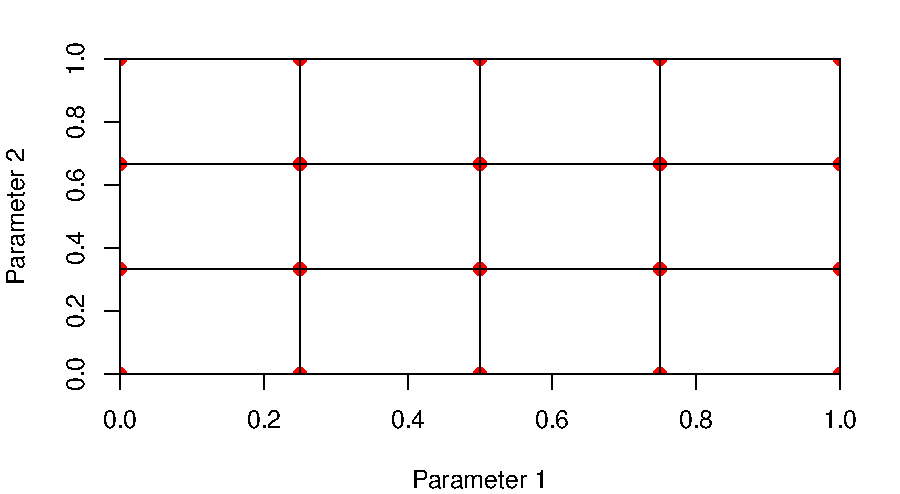
\includegraphics[width=\maxwidth]{FIGS/comp-analysis-grid-sampling-2d-example-1} 
\end{knitrout}
\end{frame}




\begin{frame}[fragile]\frametitle{Select a sampling method -- Grid sampling}
\begin{knitrout}
\definecolor{shadecolor}{rgb}{0.969, 0.969, 0.969}\color{fgcolor}\begin{kframe}
\begin{alltt}
\hldef{nb_points_per_param} \hlkwb{=} \hlnum{10}
\hldef{params.grid} \hlkwb{=} \hlkwd{expand_grid}\hldef{(}
  \hlkwc{delta} \hldef{=} \hlkwd{seq}\hldef{(params.vary}\hlopt{$}\hldef{delta[}\hlnum{1}\hldef{],}
              \hldef{params.vary}\hlopt{$}\hldef{delta[}\hlnum{2}\hldef{],}
              \hlkwc{length.out} \hldef{= nb_points_per_param),}
  \hlkwc{p} \hldef{=} \hlkwd{seq}\hldef{(params.vary}\hlopt{$}\hldef{p[}\hlnum{1}\hldef{], params.vary}\hlopt{$}\hldef{p[}\hlnum{2}\hldef{],} \hlkwc{length.out} \hldef{= nb_points_per_param),}
  \hlkwc{gamma} \hldef{=} \hlkwd{seq}\hldef{(params.vary}\hlopt{$}\hldef{gamma[}\hlnum{1}\hldef{], params.vary}\hlopt{$}\hldef{gamma[}\hlnum{2}\hldef{],} \hlkwc{length.out} \hldef{= nb_points_per_param),}
  \hlkwc{eta} \hldef{=} \hlkwd{seq}\hldef{(params.vary}\hlopt{$}\hldef{eta[}\hlnum{1}\hldef{], params.vary}\hlopt{$}\hldef{eta[}\hlnum{2}\hldef{],} \hlkwc{length.out} \hldef{= nb_points_per_param),}
  \hlkwc{beta} \hldef{=} \hlkwd{seq}\hldef{(params.vary}\hlopt{$}\hldef{beta[}\hlnum{1}\hldef{], params.vary}\hlopt{$}\hldef{beta[}\hlnum{2}\hldef{],} \hlkwc{length.out} \hldef{= nb_points_per_param))}
\end{alltt}
\end{kframe}
\end{knitrout}
\end{frame}



\begin{frame}\frametitle{Vectorised or parallel? Both?}
Functions like the ones here are easily vectorised. We show an example here
\vfill
More complex functions (for instance, requiring the use of \code{ode}) may not be vectorised and can benefit from parallelisation
\vfill
We will use the \code{parallel} package to parallelise the evaluation of the function
\vfill
It is possible to parallelise a vector function as well, but we will not do that here
\end{frame}


\begin{frame}[fragile]\frametitle{Vectorised version of the $\R_0$ function}
The first function we wrote actually works with vectors, but we need to allow S0 as an argument (as it is not varying). So we distinguish between two parameter sets, the fixed ones and the varying ones
\vfill
\begin{knitrout}
\definecolor{shadecolor}{rgb}{0.969, 0.969, 0.969}\color{fgcolor}\begin{kframe}
\begin{alltt}
\hldef{R0_SLIAR} \hlkwb{=} \hlkwa{function}\hldef{(}\hlkwc{p}\hldef{,} \hlkwc{p_fixed}\hldef{) \{}
  \hldef{OUT} \hlkwb{=} \hldef{p}\hlopt{$}\hldef{beta}\hlopt{*}\hldef{(p}\hlopt{$}\hldef{p}\hlopt{/}\hldef{p}\hlopt{$}\hldef{gamma}\hlopt{+}\hldef{p}\hlopt{$}\hldef{delta}\hlopt{*}\hldef{(}\hlnum{1}\hlopt{-}\hldef{p}\hlopt{$}\hldef{p)}\hlopt{/}\hldef{p}\hlopt{$}\hldef{eta)}\hlopt{*}\hldef{p_fixed}\hlopt{$}\hldef{S0}
  \hlkwd{return}\hldef{(OUT)}
\hldef{\}}
\hldef{R0_values} \hlkwb{=} \hlkwd{R0_SLIAR}\hldef{(params.grid, params)}
\end{alltt}
\end{kframe}
\end{knitrout}
\end{frame}


\begin{frame}[fragile]\frametitle{Now compute PRCC}
Partial rank correlation coefficients (PRCC) are a measure of the correlation between a parameter and the output of a function, controlling for the effect of the other parameters
\vfill
We make a function just to simplify the call
\vfill
\begin{knitrout}
\definecolor{shadecolor}{rgb}{0.969, 0.969, 0.969}\color{fgcolor}\begin{kframe}
\begin{alltt}
\hldef{compute_PRCC} \hlkwb{=} \hlkwa{function}\hldef{(}\hlkwc{v}\hldef{,} \hlkwc{pars}\hldef{) \{}
  \hldef{x} \hlkwb{=} \hlkwd{pcc}\hldef{(pars,} \hlkwd{as.numeric}\hldef{(v),}
          \hlkwc{rank} \hldef{=} \hlnum{TRUE}\hldef{,} \hlkwc{semi} \hldef{=} \hlnum{FALSE}\hldef{)}
  \hlkwd{return}\hldef{(x)}
\hldef{\}}
\hldef{R0_SLIAR_PRCC_grid} \hlkwb{=} \hlkwd{compute_PRCC}\hldef{(R0_values, params.grid)}
\end{alltt}
\end{kframe}
\end{knitrout}
\end{frame}

\begin{frame}[fragile]\frametitle{The PRCC values}
\begin{knitrout}
\definecolor{shadecolor}{rgb}{0.969, 0.969, 0.969}\color{fgcolor}\begin{kframe}
\begin{alltt}
\hldef{R0_SLIAR_PRCC_grid}
\end{alltt}
\begin{verbatim}
## 
## Call:
## pcc(X = pars, y = as.numeric(v), rank = TRUE, semi = FALSE)
## 
## Partial Rank Correlation Coefficients (PRCC):
##         original
## delta  0.3792029
## p      0.6462309
## gamma -0.5934708
## eta   -0.3623526
## beta   0.8778737
\end{verbatim}
\end{kframe}
\end{knitrout}
\end{frame}



\begin{frame}[fragile]\frametitle{Plotting the results using base graphics}
To make things a bit easier to read, let's sort the PRCC values in decreasing absolute value
\vfill
\begin{knitrout}
\definecolor{shadecolor}{rgb}{0.969, 0.969, 0.969}\color{fgcolor}\begin{kframe}
\begin{alltt}
\hldef{idx} \hlkwb{=} \hlkwd{order}\hldef{(}\hlkwd{abs}\hldef{(R0_SLIAR_PRCC_grid}\hlopt{$}\hldef{PRCC}\hlopt{$}\hldef{original),}
            \hlkwc{decreasing} \hldef{=} \hlnum{TRUE}\hldef{)}
\hlkwd{plot}\hldef{(R0_SLIAR_PRCC_grid}\hlopt{$}\hldef{PRCC}\hlopt{$}\hldef{original[idx],}
     \hlkwc{ylim} \hldef{=} \hlkwd{c}\hldef{(}\hlopt{-}\hlnum{1}\hldef{,}\hlnum{1}\hldef{),} \hlkwc{xaxt}\hldef{=}\hlsng{'n'}\hldef{,}
     \hlkwc{xlab} \hldef{=} \hlsng{"Parameter"}\hldef{,} \hlkwc{ylab} \hldef{=} \hlsng{"PRCC"}\hldef{,}
     \hlkwc{main} \hldef{=} \hlkwd{TeX}\hldef{(}\hlsng{"PRCC for $R_0$ - parameters sampled using a grid"}\hldef{),}
     \hlkwc{pch} \hldef{=} \hlnum{19}\hldef{,} \hlkwc{col} \hldef{=} \hlsng{"blue"}\hldef{,} \hlkwc{cex} \hldef{=} \hlnum{2}\hldef{)}
\hlkwd{axis}\hldef{(}\hlnum{1}\hldef{,} \hlkwc{at} \hldef{=} \hlnum{1}\hlopt{:}\hlkwd{length}\hldef{(idx),}
     \hlkwc{labels} \hldef{=} \hlkwd{rownames}\hldef{(R0_SLIAR_PRCC_grid}\hlopt{$}\hldef{PRCC)[idx])}
\hlkwd{abline}\hldef{(}\hlkwc{h}\hldef{=}\hlnum{0}\hldef{,} \hlkwc{lty} \hldef{=} \hlnum{3}\hldef{)}
\end{alltt}
\end{kframe}
\end{knitrout}
\end{frame}

\maxFrameImage{FIGS/comp-analysis-plot-PRCC-R0-SLIAR-grid-base-1.pdf}

\begin{frame}[fragile]\frametitle{Refining the plot a little}
Let's use different colours for the points, make their size proportional to the PRCC values and use \LaTeX for the labels
\vfill
\begin{knitrout}
\definecolor{shadecolor}{rgb}{0.969, 0.969, 0.969}\color{fgcolor}\begin{kframe}
\begin{alltt}
\hldef{colour} \hlkwb{=} \hldef{viridis}\hlopt{::}\hlkwd{viridis}\hldef{(}\hlkwd{length}\hldef{(idx))}
\hldef{labels} \hlkwb{=}  \hlkwd{sprintf}\hldef{(}\hlsng{"$\textbackslash{}\textbackslash{}%s$"}\hldef{,} \hlkwd{rownames}\hldef{(R0_SLIAR_PRCC_grid}\hlopt{$}\hldef{PRCC)[idx])}
\hldef{labels} \hlkwb{=} \hlkwd{gsub}\hldef{(}\hlsng{"\textbackslash{}\textbackslash{}\textbackslash{}\textbackslash{}p"}\hldef{,} \hlsng{"p"}\hldef{, labels)}
\hlkwd{plot}\hldef{(R0_SLIAR_PRCC_grid}\hlopt{$}\hldef{PRCC}\hlopt{$}\hldef{original[idx],}
     \hlkwc{ylim} \hldef{=} \hlkwd{c}\hldef{(}\hlopt{-}\hlnum{1}\hldef{,}\hlnum{1}\hldef{),} \hlkwc{xaxt}\hldef{=}\hlsng{'n'}\hldef{,} \hlkwc{pch} \hldef{=} \hlnum{19}\hldef{,}
     \hlkwc{xlab} \hldef{=} \hlsng{"Parameter"}\hldef{,} \hlkwc{ylab} \hldef{=} \hlsng{"PRCC"}\hldef{,}
     \hlkwc{col} \hldef{= colour,}
     \hlkwc{main} \hldef{=} \hlkwd{TeX}\hldef{(}\hlsng{"PRCC for $R_0$ - parameters sampled using a grid"}\hldef{),}
     \hlkwc{cex} \hldef{=} \hlnum{3} \hlopt{*} \hlkwd{abs}\hldef{(R0_SLIAR_PRCC_grid}\hlopt{$}\hldef{PRCC}\hlopt{$}\hldef{original)[idx])}
\hlkwd{axis}\hldef{(}\hlnum{1}\hldef{,} \hlkwc{at} \hldef{=} \hlnum{1}\hlopt{:}\hlkwd{length}\hldef{(idx),} \hlkwc{labels} \hldef{=} \hlkwd{TeX}\hldef{(labels))}
\hlkwd{abline}\hldef{(}\hlkwc{h}\hldef{=}\hlnum{0}\hldef{,} \hlkwc{lty} \hldef{=} \hlnum{3}\hldef{)}
\end{alltt}
\end{kframe}
\end{knitrout}
\end{frame}

\maxFrameImage{FIGS/comp-analysis-plot-PRCC-R0-SLIAR-grid-2-1.pdf}


\begin{frame}[fragile]\frametitle{Plotting the results using ggplot2}
\begin{knitrout}
\definecolor{shadecolor}{rgb}{0.969, 0.969, 0.969}\color{fgcolor}\begin{kframe}
\begin{alltt}
\hldef{df} \hlkwb{=} \hlkwd{data.frame}\hldef{(}\hlkwc{Parameter} \hldef{=} \hlkwd{rownames}\hldef{(R0_SLIAR_PRCC_grid}\hlopt{$}\hldef{PRCC)[idx],}
                \hlkwc{PRCC} \hldef{= R0_SLIAR_PRCC_grid}\hlopt{$}\hldef{PRCC}\hlopt{$}\hldef{original[idx])}
\hlkwd{ggplot}\hldef{(df,} \hlkwd{aes}\hldef{(}\hlkwc{x} \hldef{= Parameter,} \hlkwc{y} \hldef{= PRCC))} \hlopt{+}
  \hlkwd{geom_point}\hldef{(}\hlkwc{colour} \hldef{=} \hlsng{"blue"}\hldef{,} \hlkwc{size} \hldef{=} \hlnum{3}\hldef{)} \hlopt{+}
  \hlkwd{geom_hline}\hldef{(}\hlkwc{yintercept} \hldef{=} \hlnum{0}\hldef{,} \hlkwc{linetype} \hldef{=} \hlsng{"dotted"}\hldef{)} \hlopt{+}
  \hlkwd{theme}\hldef{(}\hlkwc{axis.text.x} \hldef{=} \hlkwd{element_text}\hldef{(}\hlkwc{angle} \hldef{=} \hlnum{45}\hldef{,} \hlkwc{hjust} \hldef{=} \hlnum{1}\hldef{))} \hlopt{+}
  \hlkwd{theme_minimal}\hldef{()}
\end{alltt}
\end{kframe}
\end{knitrout}
\end{frame}

\maxFrameImage{FIGS/comp-analysis-plot-PRCC-R0-SLIAR-grid-ggplot2-1.pdf}


\begin{frame}\frametitle{The problem with grid sampling}
Suppose we decide that since 100,000 evaluations are done easily, we can afford to do 1,000,000 evaluations
\vfill
How do we implement that?
\vfill
We have
\[
1,000,000^{1/5} \simeq 15.8489
\]
so we could decide to cut each range in 16 parts
\vfill
If the range of each parameter is relatively large, this could quickly become unmanageable
\end{frame}

\begin{frame}[fragile]\frametitle{What if I do want grid sampling nonetheless?}
The function \code{parameterSets} from the \code{sensitivity} package can be used to generate a grid of parameter sets
\vfill
\begin{knitrout}
\definecolor{shadecolor}{rgb}{0.969, 0.969, 0.969}\color{fgcolor}\begin{kframe}
\begin{alltt}
\hldef{nb_samples} \hlkwb{=} \hlnum{1000000}
\hldef{length_grid_side} \hlkwb{=} \hlkwd{floor}\hldef{(nb_samples}\hlopt{^}\hldef{(}\hlnum{1}\hlopt{/}\hlnum{5}\hldef{))}
\hldef{params.grid} \hlkwb{=} \hlkwd{parameterSets}\hldef{(}\hlkwc{par.ranges} \hldef{= params.vary,}
                             \hlkwc{samples} \hldef{=} \hlkwd{rep}\hldef{(length_grid_side,} \hlnum{5}\hldef{),}
                             \hlkwc{method} \hldef{=} \hlsng{"grid"}\hldef{)}
\hldef{params.grid} \hlkwb{=} \hlkwd{as.data.frame}\hldef{(params.grid)}
\hlkwd{colnames}\hldef{(params.grid)} \hlkwb{=} \hlkwd{names}\hldef{(params.vary)}
\hldef{R0_values} \hlkwb{=} \hlkwd{R0_SLIAR}\hldef{(params.grid, params)}
\hldef{R0_SLIAR_PRCC_grid_2} \hlkwb{=} \hlkwd{compute_PRCC}\hldef{(R0_values, params.grid)}
\end{alltt}
\end{kframe}
\end{knitrout}
\vfill
You can also use \code{method="innergrid"} to generate a grid of parameter sets that are offset from the sides of the hypecube
\end{frame}



%%%%%%%%%%%%%%%%%%%%%%%
\subsubsection{Sobol sampling}
\newSubSubSectionSlide{FIGS/Gemini_Generated_Image_hfkrgfhfkrgfhfkr.jpeg}


\begin{frame}[fragile]\frametitle{Sobol sampling (20 samples)}
\begin{knitrout}
\definecolor{shadecolor}{rgb}{0.969, 0.969, 0.969}\color{fgcolor}
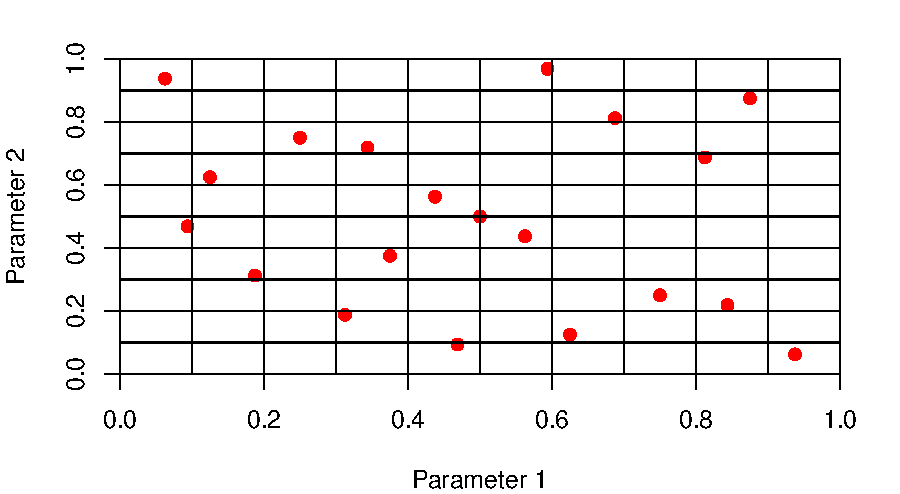
\includegraphics[width=\maxwidth]{FIGS/comp-analysis-sobol-sampling-2d-example-1} 
\end{knitrout}
\end{frame}


\begin{frame}[fragile]\frametitle{Select a sampling method -- Sobol}
This uses the \code{sensitivity} package
\vfill
\begin{knitrout}
\definecolor{shadecolor}{rgb}{0.969, 0.969, 0.969}\color{fgcolor}\begin{kframe}
\begin{alltt}
\hldef{nb_samples} \hlkwb{=} \hlnum{100000}
\hldef{params.sobol} \hlkwb{=} \hlkwd{parameterSets}\hldef{(}\hlkwc{par.ranges} \hldef{= params.vary,}
                             \hlkwc{samples} \hldef{= nb_samples,}
                             \hlkwc{method} \hldef{=} \hlsng{"sobol"}\hldef{)}
\hldef{params.sobol} \hlkwb{=} \hlkwd{as.data.frame}\hldef{(params.sobol)}
\hlkwd{colnames}\hldef{(params.sobol)} \hlkwb{=} \hlkwd{names}\hldef{(params.vary)}
\end{alltt}
\end{kframe}
\end{knitrout}
\end{frame}

\begin{frame}[fragile]\frametitle{Compute PRCC with Sobol sampling}
Partial rank correlation coefficients (PRCC) are a measure of the correlation between a parameter and the output of a function, controlling for the effect of the other parameters
\vfill
\begin{knitrout}
\definecolor{shadecolor}{rgb}{0.969, 0.969, 0.969}\color{fgcolor}\begin{kframe}
\begin{alltt}
\hldef{R0_values} \hlkwb{=} \hlkwd{R0_SLIAR}\hldef{(params.sobol, params)}
\hldef{compute_PRCC} \hlkwb{=} \hlkwa{function}\hldef{(}\hlkwc{v}\hldef{,} \hlkwc{pars}\hldef{) \{}
  \hldef{x} \hlkwb{=} \hlkwd{pcc}\hldef{(pars,} \hlkwd{as.numeric}\hldef{(v),}
          \hlkwc{rank} \hldef{=} \hlnum{TRUE}\hldef{,} \hlkwc{semi} \hldef{=} \hlnum{FALSE}\hldef{)}
  \hlkwd{return}\hldef{(x)}
\hldef{\}}
\hldef{R0_SLIAR_PRCC_sobol} \hlkwb{=} \hlkwd{compute_PRCC}\hldef{(R0_values, params.sobol)}
\end{alltt}
\end{kframe}
\end{knitrout}
\end{frame}

\begin{frame}[fragile]\frametitle{The PRCC values}
\begin{knitrout}
\definecolor{shadecolor}{rgb}{0.969, 0.969, 0.969}\color{fgcolor}\begin{kframe}
\begin{alltt}
\hldef{R0_SLIAR_PRCC_sobol}
\end{alltt}
\begin{verbatim}
## 
## Call:
## pcc(X = pars, y = as.numeric(v), rank = TRUE, semi = FALSE)
## 
## Partial Rank Correlation Coefficients (PRCC):
##         original
## delta  0.4129675
## p      0.7018390
## gamma -0.6578156
## eta   -0.3885156
## beta   0.8996126
\end{verbatim}
\end{kframe}
\end{knitrout}
\end{frame}



\begin{frame}[fragile]\frametitle{Plotting the results using base graphics}
\begin{knitrout}
\definecolor{shadecolor}{rgb}{0.969, 0.969, 0.969}\color{fgcolor}\begin{kframe}
\begin{alltt}
\hldef{idx} \hlkwb{=} \hlkwd{order}\hldef{(}\hlkwd{abs}\hldef{(R0_SLIAR_PRCC_sobol}\hlopt{$}\hldef{PRCC}\hlopt{$}\hldef{original),}
            \hlkwc{decreasing} \hldef{=} \hlnum{TRUE}\hldef{)}
\hldef{colour} \hlkwb{=} \hldef{viridis}\hlopt{::}\hlkwd{viridis}\hldef{(}\hlkwd{length}\hldef{(idx))}
\hldef{labels} \hlkwb{=}  \hlkwd{sprintf}\hldef{(}\hlsng{"$\textbackslash{}\textbackslash{}%s$"}\hldef{,} \hlkwd{rownames}\hldef{(R0_SLIAR_PRCC_sobol}\hlopt{$}\hldef{PRCC)[idx])}
\hldef{labels} \hlkwb{=} \hlkwd{gsub}\hldef{(}\hlsng{"\textbackslash{}\textbackslash{}\textbackslash{}\textbackslash{}p"}\hldef{,} \hlsng{"p"}\hldef{, labels)}
\hlkwd{plot}\hldef{(R0_SLIAR_PRCC_sobol}\hlopt{$}\hldef{PRCC}\hlopt{$}\hldef{original[idx],}
     \hlkwc{ylim} \hldef{=} \hlkwd{c}\hldef{(}\hlopt{-}\hlnum{1}\hldef{,}\hlnum{1}\hldef{),} \hlkwc{xaxt}\hldef{=}\hlsng{'n'}\hldef{,} \hlkwc{pch} \hldef{=} \hlnum{19}\hldef{,}
     \hlkwc{xlab} \hldef{=} \hlsng{"Parameter"}\hldef{,} \hlkwc{ylab} \hldef{=} \hlsng{"PRCC"}\hldef{,}
     \hlkwc{col} \hldef{= colour,}
     \hlkwc{main} \hldef{=} \hlkwd{TeX}\hldef{(}\hlsng{"PRCC for $R_0$ - parameters sampled using Sobol"}\hldef{),}
     \hlkwc{cex} \hldef{=} \hlnum{3} \hlopt{*} \hlkwd{abs}\hldef{(R0_SLIAR_PRCC_sobol}\hlopt{$}\hldef{PRCC}\hlopt{$}\hldef{original)[idx])}
\hlkwd{axis}\hldef{(}\hlnum{1}\hldef{,} \hlkwc{at} \hldef{=} \hlnum{1}\hlopt{:}\hlkwd{length}\hldef{(idx),} \hlkwc{labels} \hldef{=} \hlkwd{TeX}\hldef{(labels))}
\hlkwd{abline}\hldef{(}\hlkwc{h}\hldef{=}\hlnum{0}\hldef{,} \hlkwc{lty} \hldef{=} \hlnum{3}\hldef{)}
\end{alltt}
\end{kframe}
\end{knitrout}
\end{frame}

\maxFrameImage{FIGS/comp-analysis-plot-PRCC-R0-SLIAR-2-1.pdf}


\begin{frame}[fragile]\frametitle{Plotting the results using ggplot2}
\begin{knitrout}
\definecolor{shadecolor}{rgb}{0.969, 0.969, 0.969}\color{fgcolor}\begin{kframe}
\begin{alltt}
\hldef{df} \hlkwb{=} \hlkwd{data.frame}\hldef{(}\hlkwc{Parameter} \hldef{=} \hlkwd{rownames}\hldef{(R0_SLIAR_PRCC_sobol}\hlopt{$}\hldef{PRCC)[idx],}
                \hlkwc{PRCC} \hldef{= R0_SLIAR_PRCC_sobol}\hlopt{$}\hldef{PRCC}\hlopt{$}\hldef{original[idx])}
\hlkwd{ggplot}\hldef{(df,} \hlkwd{aes}\hldef{(}\hlkwc{x} \hldef{= Parameter,} \hlkwc{y} \hldef{= PRCC))} \hlopt{+}
  \hlkwd{geom_point}\hldef{(}\hlkwc{colour} \hldef{=} \hlsng{"blue"}\hldef{,} \hlkwc{size} \hldef{=} \hlnum{3}\hldef{)} \hlopt{+}
  \hlkwd{geom_hline}\hldef{(}\hlkwc{yintercept} \hldef{=} \hlnum{0}\hldef{,} \hlkwc{linetype} \hldef{=} \hlsng{"dotted"}\hldef{)} \hlopt{+}
  \hlkwd{theme}\hldef{(}\hlkwc{axis.text.x} \hldef{=} \hlkwd{element_text}\hldef{(}\hlkwc{angle} \hldef{=} \hlnum{45}\hldef{,} \hlkwc{hjust} \hldef{=} \hlnum{1}\hldef{))} \hlopt{+}
  \hlkwd{theme_minimal}\hldef{()}
\end{alltt}
\end{kframe}
\end{knitrout}
\end{frame}

\maxFrameImage{FIGS/comp-analysis-plot-PRCC-R0-SLIAR-ggplot2-1.pdf}


%%%%%%%%%%%%%%%%%%%%%%%
\subsubsection{Latin Hypercube Sampling}
\newSubSubSectionSlide{FIGS/Gemini_Generated_Image_i0pbri0pbri0pbri.jpeg}

\begin{frame}[fragile]\frametitle{Select a sampling method -- Latin Hypercube}
This is another method to sample the parameter space
\vfill
\begin{quote}
\href{https://en.wikipedia.org/wiki/Latin_hypercube_sampling}{From Wikipedia}
In the context of statistical sampling, a square grid containing sample positions is a Latin square if (and only if) there is only one sample in each row and each column. A Latin hypercube is the generalisation of this concept to an arbitrary number of dimensions, whereby each sample is the only one in each axis-aligned hyperplane containing it.
\end{quote}
\end{frame}

\begin{frame}[fragile]\frametitle{Latin hypercube sampling (20 samples)}
\begin{knitrout}
\definecolor{shadecolor}{rgb}{0.969, 0.969, 0.969}\color{fgcolor}
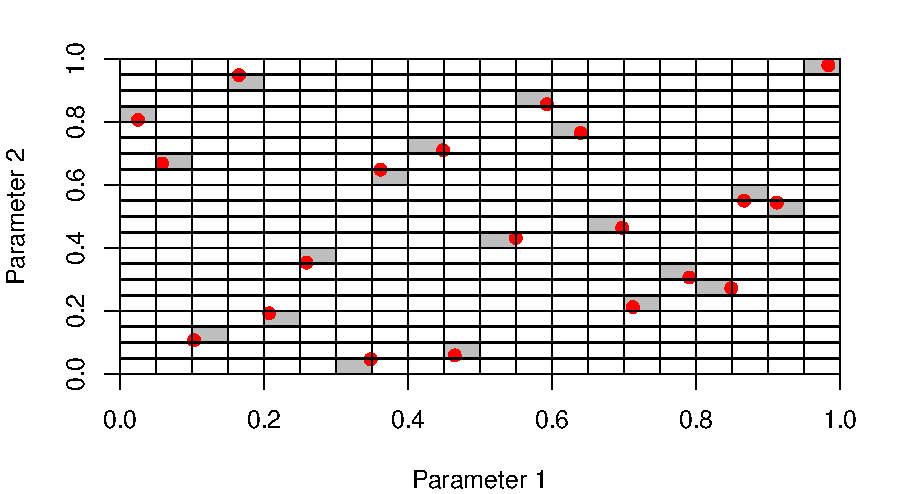
\includegraphics[width=\maxwidth]{FIGS/comp-analysis-lhs-sampling-2d-example-1} 
\end{knitrout}
\end{frame}

\begin{frame}[fragile]\frametitle{Select a sampling method -- Latin Hypercube}
Call the function with arguments for the number of samples and the number of parameters
\begin{knitrout}
\definecolor{shadecolor}{rgb}{0.969, 0.969, 0.969}\color{fgcolor}\begin{kframe}
\begin{alltt}
\hldef{params.lhs} \hlkwb{=} \hldef{lhs}\hlopt{::}\hlkwd{randomLHS}\hldef{(nb_samples,} \hlkwd{length}\hldef{(params.vary))}
\hldef{params.lhs} \hlkwb{=} \hlkwd{as.data.frame}\hldef{(params.lhs)}
\hlkwd{colnames}\hldef{(params.lhs)} \hlkwb{=} \hlkwd{names}\hldef{(params.vary)}
\hlkwd{head}\hldef{(params.lhs)}
\end{alltt}
\begin{verbatim}
##       delta          p      gamma       eta      beta
## 1 0.2196281 0.65674325 0.47224889 0.6055470 0.4467295
## 2 0.3923825 0.70044379 0.18594261 0.3877079 0.6882853
## 3 0.1343409 0.23472237 0.40297181 0.6030566 0.9984018
## 4 0.9139961 0.09964145 0.05388207 0.9800108 0.7528688
## 5 0.5624563 0.42259898 0.19264973 0.6475799 0.9647556
## 6 0.3854645 0.68503310 0.40032684 0.9348806 0.3037644
\end{verbatim}
\end{kframe}
\end{knitrout}
\vfill
Results are uniform on $[0,1]$ for each parameter and need to be transformed prior to use
\end{frame}

\begin{frame}[fragile]\frametitle{Transforming the uniform distribution}
Suppose values $\xi$ uniformly distributed on $[0,1]$ are to be transformed to the range $[x_{\min},x_{\max}]$
\begin{align*}
x = x_{\min} + \xi (x_{\max} - x_{\min})
\end{align*}
\vfill
\begin{knitrout}
\definecolor{shadecolor}{rgb}{0.969, 0.969, 0.969}\color{fgcolor}\begin{kframe}
\begin{alltt}
\hlkwa{for} \hldef{(c} \hlkwa{in} \hlnum{1}\hlopt{:}\hlkwd{length}\hldef{(params.vary)) \{}
  \hldef{params.lhs[,c]} \hlkwb{=} \hldef{params.vary[[c]][}\hlnum{1}\hldef{]} \hlopt{+} \hldef{params.lhs[,c]} \hlopt{*}
    \hldef{(params.vary[[c]][}\hlnum{2}\hldef{]} \hlopt{-} \hldef{params.vary[[c]][}\hlnum{1}\hldef{])}
\hldef{\}}
\hldef{R0_values} \hlkwb{=} \hlkwd{R0_SLIAR}\hldef{(params.lhs, params)}
\hldef{R0_SLIAR_PRCC_lhs} \hlkwb{=} \hlkwd{compute_PRCC}\hldef{(R0_values, params.lhs)}
\end{alltt}
\end{kframe}
\end{knitrout}
\end{frame}


\begin{frame}[fragile]\frametitle{Plotting the results using base graphics}
\begin{knitrout}
\definecolor{shadecolor}{rgb}{0.969, 0.969, 0.969}\color{fgcolor}\begin{kframe}
\begin{alltt}
\hldef{idx} \hlkwb{=} \hlkwd{order}\hldef{(}\hlkwd{abs}\hldef{(R0_SLIAR_PRCC_lhs}\hlopt{$}\hldef{PRCC}\hlopt{$}\hldef{original),}
            \hlkwc{decreasing} \hldef{=} \hlnum{TRUE}\hldef{)}
\hldef{colour} \hlkwb{=} \hldef{viridis}\hlopt{::}\hlkwd{viridis}\hldef{(}\hlkwd{length}\hldef{(idx))}
\hldef{labels} \hlkwb{=}  \hlkwd{sprintf}\hldef{(}\hlsng{"$\textbackslash{}\textbackslash{}%s$"}\hldef{,} \hlkwd{rownames}\hldef{(R0_SLIAR_PRCC_lhs}\hlopt{$}\hldef{PRCC)[idx])}
\hldef{labels} \hlkwb{=} \hlkwd{gsub}\hldef{(}\hlsng{"\textbackslash{}\textbackslash{}\textbackslash{}\textbackslash{}p"}\hldef{,} \hlsng{"p"}\hldef{, labels)}
\hlkwd{plot}\hldef{(R0_SLIAR_PRCC_lhs}\hlopt{$}\hldef{PRCC}\hlopt{$}\hldef{original[idx],}
     \hlkwc{ylim} \hldef{=} \hlkwd{c}\hldef{(}\hlopt{-}\hlnum{1}\hldef{,}\hlnum{1}\hldef{),} \hlkwc{xaxt}\hldef{=}\hlsng{'n'}\hldef{,} \hlkwc{pch} \hldef{=} \hlnum{19}\hldef{,}
     \hlkwc{xlab} \hldef{=} \hlsng{"Parameter"}\hldef{,} \hlkwc{ylab} \hldef{=} \hlsng{"PRCC"}\hldef{,}
     \hlkwc{main} \hldef{=} \hlkwd{TeX}\hldef{(}\hlsng{"PRCC for $R_0$ with parameters sampled using LHS"}\hldef{),}
     \hlkwc{col} \hldef{= colour,}
     \hlkwc{cex} \hldef{=} \hlnum{3} \hlopt{*} \hlkwd{abs}\hldef{(R0_SLIAR_PRCC_lhs}\hlopt{$}\hldef{PRCC}\hlopt{$}\hldef{original)[idx])}
\hlkwd{axis}\hldef{(}\hlnum{1}\hldef{,} \hlkwc{at} \hldef{=} \hlnum{1}\hlopt{:}\hlkwd{length}\hldef{(idx),} \hlkwc{labels} \hldef{=} \hlkwd{TeX}\hldef{(labels))}
\hlkwd{abline}\hldef{(}\hlkwc{h}\hldef{=}\hlnum{0}\hldef{,} \hlkwc{lty} \hldef{=} \hlnum{3}\hldef{)}
\end{alltt}
\end{kframe}
\end{knitrout}
\end{frame}

\maxFrameImage{FIGS/comp-analysis-plot-PRCC-R0-SLIAR-lhs-1.pdf}

%%%%%%%%%%%%%%%%%%%%%%%
\subsubsection{Comparing results}
\newSubSubSectionSlide{FIGS/Gemini_Generated_Image_a2j2lja2j2lja2j2.jpeg}
\begin{frame}[fragile]\frametitle{Comparing the PRCC values}
\begin{kframe}
\begin{alltt}
\hldef{R0_SLIAR_PRCC} \hlkwb{=} \hlkwd{cbind}\hldef{(R0_SLIAR_PRCC_grid}\hlopt{$}\hldef{PRCC}\hlopt{$}\hldef{original,}
                \hldef{R0_SLIAR_PRCC_grid_2}\hlopt{$}\hldef{PRCC}\hlopt{$}\hldef{original,}
                \hldef{R0_SLIAR_PRCC_sobol}\hlopt{$}\hldef{PRCC}\hlopt{$}\hldef{original,}
                \hldef{R0_SLIAR_PRCC_lhs}\hlopt{$}\hldef{PRCC}\hlopt{$}\hldef{original)}
\hlkwd{rownames}\hldef{(R0_SLIAR_PRCC)} \hlkwb{=} \hlkwd{rownames}\hldef{(R0_SLIAR_PRCC_grid}\hlopt{$}\hldef{PRCC)}
\hlkwd{colnames}\hldef{(R0_SLIAR_PRCC)} \hlkwb{=} \hlkwd{c}\hldef{(}\hlsng{"Grid 1"}\hldef{,} \hlsng{"Grid 2"}\hldef{,} \hlsng{"Sobol"}\hldef{,} \hlsng{"LHS"}\hldef{)}
\hldef{knitr}\hlopt{::}\hlkwd{kable}\hldef{(R0_SLIAR_PRCC,} \hlkwc{digits} \hldef{=} \hlnum{3}\hldef{,} \hlkwc{booktabs} \hldef{=} \hlnum{TRUE}\hldef{)}
\end{alltt}
\end{kframe}
\begin{tabular}{lrrrr}
\toprule
  & Grid 1 & Grid 2 & Sobol & LHS\\
\midrule
delta & 0.379 & 0.389 & 0.413 & 0.409\\
p & 0.646 & 0.663 & 0.702 & 0.704\\
gamma & -0.593 & -0.614 & -0.658 & -0.660\\
eta & -0.362 & -0.370 & -0.389 & -0.390\\
beta & 0.878 & 0.885 & 0.900 & 0.900\\
\bottomrule
\end{tabular}


\end{frame}


\begin{frame}\frametitle{One last remark on sensitivity}
We have used $\gamma$ and $\eta$
\vfill
We saw when plotting $\R_0$ as a function of $\gamma$ that the situation is very different when using $\gamma$ and $1/\gamma$
\vfill
The same is true, to a lesser extent, of $\eta$ and $1/\eta$
\vfill
We would therefore get a very different picture if we considered $1/\gamma$ and $1/\eta$ for the sensitivity analysis 
\end{frame}


\begin{frame}\frametitle{Nobody expects the Spanish Inquisition!}
Here, we used PRCC. There are many other types of sensititivities that can be computed
\vfill
The \code{sensitivity} packages has quite an array of these. See the package documentation for details
\vfill
There are other \code{R} packages that also do sensitivity analysis
\end{frame}

%%%%%%%%%%%%%%%%%%%%%%%
\subsubsection{Using a parallel version}
\newSubSubSectionSlide{FIGS/Gemini_Generated_Image_hgadozhgadozhgad.jpeg}

\begin{frame}\frametitle{Why parallelise?}
Numerical problems like the evaluation of a function at a bunch of points in parameter space when all evaluations are independent from one another are \defword{embarassingly parallel}
\vfill
In the case of the PRCC for $\R_0$ like here, parallel is not necessarily a good idea, as there is a lot of overhead
\vfill
However, if you are computing the response of a more complex function, e.g., simulating the solutions to an ODE then performing a bunch of computations, then parallelising can greatly speed stuff up
\end{frame}


\begin{frame}[fragile]\frametitle{Setting up the parallel version}
The easiest way is to use \code{parLapply}. For this, we need a list in which each entry is a list with a specific point in parameter space
\vfill
\begin{knitrout}
\definecolor{shadecolor}{rgb}{0.969, 0.969, 0.969}\color{fgcolor}\begin{kframe}
\begin{alltt}
\hldef{params.sobol.list} \hlkwb{=} \hlkwd{split}\hldef{(params.sobol,} \hlkwd{seq}\hldef{(}\hlkwd{nrow}\hldef{(params.sobol)))}
\hlkwd{head}\hldef{(params.sobol.list,} \hlkwc{n} \hldef{=} \hlnum{2}\hldef{)}
\end{alltt}
\begin{verbatim}
## $`1`
##   delta   p gamma       eta        beta
## 1 0.525 0.5   0.3 0.5714286 0.002527528
## 
## $`2`
##    delta    p gamma       eta        beta
## 2 0.7625 0.25   0.4 0.3571429 0.003766266
\end{verbatim}
\end{kframe}
\end{knitrout}
\end{frame}

\begin{frame}[fragile]\frametitle{Testing iteratively first}
If your code is going to run in parallel using \code{parLapply}, it also needs to run sequentially using \code{lapply}
\vfill
Using \code{lapply} also is good to debug, as debugging parallel code is not easy
\vfill
\begin{knitrout}
\definecolor{shadecolor}{rgb}{0.969, 0.969, 0.969}\color{fgcolor}\begin{kframe}
\begin{alltt}
\hldef{R0_values} \hlkwb{=} \hlkwd{lapply}\hldef{(}\hlkwc{X} \hldef{= params.sobol.list,}
                   \hlkwc{FUN} \hldef{=} \hlkwa{function}\hldef{(}\hlkwc{x}\hldef{)} \hlkwd{R0_SLIAR}\hldef{(x, params))}
\hlkwd{head}\hldef{(R0_values,} \hlkwc{n} \hldef{=} \hlnum{2}\hldef{)}
\end{alltt}
\begin{verbatim}
## $`1`
## [1] 5.368255
## 
## $`2`
## [1] 8.376266
\end{verbatim}
\end{kframe}
\end{knitrout}
\end{frame}


\begin{frame}\frametitle{Note the little trick here}
The function \code{R0\_SLIAR} takes two arguments, \code{p} and \code{p\_fixed}
\vfill
However, \code{lapply} (or \code{parLapply} later) only allow dependence on a single variable
\vfill
Suppose we have a function \code{f(a,b)}
\vfill
We use the construct \code{function(x) f(x,b)} to make \code{f} depend only its first argument
\vfill
Similarly, \code{function(x) f(a,x)} would make \code{f} depend only on its second argument
\end{frame}

\begin{frame}[fragile]\frametitle{Sequential works, let's go parallel}
To run your code in parallel using \code{parLapply}, you need several steps:
\vfill
\begin{itemize}
\item Create a \emph{cluster}, i.e., a group of \emph{workers} that will each execute the function passed as argument to \code{parLapply} (\code{R0\_SLIAR} here). Typically, you want to use all compute cores but one (unless you are on a headless server), otherwise your machine may become unresponsive
\vfill
\item Provide each worker with all they need to execute the function. Each worker is an instance of \code{R} running independently
\vfill
\item Call \code{parLapply} to have the workers run the code
\vfill
\item Close the cluster to ``free up'' the workers
\end{itemize}
\end{frame}


\begin{frame}[fragile]\frametitle{Let's go parallel! (and time our run)}
\begin{knitrout}
\definecolor{shadecolor}{rgb}{0.969, 0.969, 0.969}\color{fgcolor}\begin{kframe}
\begin{alltt}
\hldef{nb_cores} \hlkwb{<-} \hldef{parallel}\hlopt{::}\hlkwd{detectCores}\hldef{()} \hlopt{-} \hlnum{1}
\hldef{nb_cores} \hlkwb{<-} \hlkwd{ifelse}\hldef{(nb_cores} \hlopt{>} \hlnum{122}\hldef{,} \hlnum{122}\hldef{, nb_cores)}
\hldef{tictoc}\hlopt{::}\hlkwd{tic}\hldef{(}\hlsng{"whole parallel phase"}\hldef{)}
\hldef{cl} \hlkwb{<-} \hldef{parallel}\hlopt{::}\hlkwd{makeCluster}\hldef{(nb_cores)}
\hldef{parallel}\hlopt{::}\hlkwd{clusterExport}\hldef{(cl,} \hlkwd{c}\hldef{(}\hlsng{"params"}\hldef{,} \hlsng{"R0_SLIAR"}\hldef{))}
\hldef{tictoc}\hlopt{::}\hlkwd{tic}\hldef{(}\hlsng{"parLapply"}\hldef{)}
\hldef{result} \hlkwb{=} \hldef{parallel}\hlopt{::}\hlkwd{parLapply}\hldef{(}\hlkwc{cl} \hldef{= cl,} \hlkwc{X} \hldef{= params.sobol.list,}
                             \hlkwc{fun} \hldef{=}  \hlkwa{function}\hldef{(}\hlkwc{x}\hldef{)} \hlkwd{R0_SLIAR}\hldef{(x, params))}
\hldef{tictoc}\hlopt{::}\hlkwd{toc}\hldef{()}
\end{alltt}
\begin{verbatim}
## parLapply: 0.751 sec elapsed
\end{verbatim}
\begin{alltt}
\hldef{parallel}\hlopt{::}\hlkwd{stopCluster}\hldef{(cl)}
\hldef{tictoc}\hlopt{::}\hlkwd{toc}\hldef{()}
\end{alltt}
\begin{verbatim}
## whole parallel phase: 1.133 sec elapsed
\end{verbatim}
\end{kframe}
\end{knitrout}
\end{frame}

\begin{frame}[fragile]\frametitle{Just for comparison}
\begin{knitrout}
\definecolor{shadecolor}{rgb}{0.969, 0.969, 0.969}\color{fgcolor}\begin{kframe}
\begin{alltt}
\hldef{tictoc}\hlopt{::}\hlkwd{tic}\hldef{(}\hlsng{"lapply"}\hldef{)}
\hldef{result} \hlkwb{=} \hlkwd{lapply}\hldef{(}\hlkwc{X} \hldef{= params.sobol.list,}
                \hlkwc{FUN} \hldef{=}  \hlkwa{function}\hldef{(}\hlkwc{x}\hldef{)} \hlkwd{R0_SLIAR}\hldef{(x, params))}
\hldef{tictoc}\hlopt{::}\hlkwd{toc}\hldef{()}
\end{alltt}
\begin{verbatim}
## lapply: 1.031 sec elapsed
\end{verbatim}
\begin{alltt}
\hldef{tictoc}\hlopt{::}\hlkwd{tic}\hldef{(}\hlsng{"vectorised"}\hldef{)}
\hldef{result} \hlkwb{=} \hlkwd{R0_SLIAR}\hldef{(params.sobol, params)}
\hldef{tictoc}\hlopt{::}\hlkwd{toc}\hldef{()}
\end{alltt}
\begin{verbatim}
## vectorised: 0.002 sec elapsed
\end{verbatim}
\end{kframe}
\end{knitrout}
\end{frame}


\begin{frame}\frametitle{Remarks about running in parallel}
Here, the gain was not massive and the overhead of setting up the cluster was not negligible (cluster setup is sequential so setup time depends on the number of cores)
\vfill
One of the machines I run this on has 128 threads. \code{R} has hard coded limit of 128 threads and uses a few of them for other things $\implies$ limit to 122 threads. If you try to use more, your parallel code will not run
\vfill
If you want to get rid of this limitation, you need to recompile \code{R} with a higher limit. See a blog post I made about this (\href{https://julien-arino.github.io/blog/2023/R-on-raspberri-pi-and-more-than-128-threads/}{link})
\vfill
That post also explains how to set up a cluster using multiple machines
\end{frame}

%%%%%%%%%%%%%%%%%%%%%%%
%%%%%%%%%%%%%%%%%%%%%%%
\subsection{Now repeat everything for the SLIARVS model}
\newSubSectionSlide{FIGS/Gemini_Generated_Image_l5l0q6l5l0q6l5l0.jpeg}

%%%%%%%%%%%%%%%%%%%%%%%
%%%%%%%%%%%%%%%%%%%%%%%
%%%%%%%%%%%%%%%%%%%%%%%
%%%%%%%%%%%%%%%%%%%%%%%
\section{Considerations on the final size}
\newSectionSlide{FIGS/Gemini_Generated_Image_1vpz11vpz11vpz11.jpeg}


%%%%%%%%%%%%%%%%%%%%%%%
%%%%%%%%%%%%%%%%%%%%%%%
%%%%%%%%%%%%%%%%%%%%%%%
%%%%%%%%%%%%%%%%%%%%%%%
\begin{frame}[fragile]\frametitle{\textsc{Can I have this wrapped up to go?}}
To finish, we use the command \code{purl} to generate an \code{R} file (\code{basic-computational-analysis.R}) in the CODE directory with all the code chunks in this \code{Rnw} file
\vfill
\begin{knitrout}
\definecolor{shadecolor}{rgb}{0.969, 0.969, 0.969}\color{fgcolor}\begin{kframe}
\begin{alltt}
\hlcom{# From https://stackoverflow.com/questions/36868287/purl-within-knit-duplicate-label-error}
\hldef{rmd_chunks_to_r_temp} \hlkwb{<-} \hlkwa{function}\hldef{(}\hlkwc{file}\hldef{)\{}
  \hldef{callr}\hlopt{::}\hlkwd{r}\hldef{(}\hlkwa{function}\hldef{(}\hlkwc{file}\hldef{,} \hlkwc{temp}\hldef{)\{}
    \hldef{out_file} \hlkwb{=} \hlkwd{sprintf}\hldef{(}\hlsng{"../CODE/%s"}\hldef{,} \hlkwd{gsub}\hldef{(}\hlsng{".Rnw"}\hldef{,} \hlsng{".R"}\hldef{, file))}
    \hldef{knitr}\hlopt{::}\hlkwd{purl}\hldef{(file,} \hlkwc{output} \hldef{= out_file,} \hlkwc{documentation} \hldef{=} \hlnum{1}\hldef{)}
  \hldef{\},} \hlkwc{args} \hldef{=} \hlkwd{list}\hldef{(file))}
\hldef{\}}
\hlkwd{rmd_chunks_to_r_temp}\hldef{(}\hlsng{"basic-computational-analysis-1-functions.Rnw"}\hldef{)}
\end{alltt}
\begin{verbatim}
## [1] "../CODE/basic-computational-analysis-1-functions.R"
\end{verbatim}
\end{kframe}
\end{knitrout}
\end{frame}

\begin{frame}[fragile]\frametitle{About that \code{R} file}
Source the file \code{basic-computational-analysis-1-functions.R} (in the \code{CODE} directory) in \code{R} to reproduce all the results in these slides
\vfill
Some small changes are required; for instance, when sourcing (instead of knitting or interactively), \code{ggplot} figures are created but not printed, so in the \code{R} file, you need to print them ``manually''
\vfill
\begin{knitrout}
\definecolor{shadecolor}{rgb}{0.969, 0.969, 0.969}\color{fgcolor}\begin{kframe}
\begin{alltt}
\hldef{pp} \hlkwb{=} \hlkwd{ggplot}\hldef{(...)}
\hlkwd{print}\hldef{(pp)}
\end{alltt}
\end{kframe}
\end{knitrout}
\end{frame}

\end{document}
